%pdflatex
%\RequirePackage[l2tabu,orthodox]{nag} % This package helps prevent you from doing things wrong.

%\documentclass[12pt,a4paper,fleqn]{article}
\documentclass[10pt,review]{elsarticle}
%\documentclass[final,5p,times,twocolumn]{elsarticle}

% \usepackage{ifluatex}
% \ifluatex
%   \usepackage{fontspec}
%   %\setmainfont[Ligatures=TeX]{xits}
%   %\setmathfont[math-style=ISO]{xits-math}
%   \setmainfont[Ligatures=TeX]{Latin Modern Roman}
%   \fontspec[SmallCapsFeatures={Letters=SmallCaps}]{Latin Modern Roman}
% \else
  \usepackage[utf8]{inputenc}
% \fi

\usepackage{lineno}
%\usepackage{refcheck}
%\usepackage[margin=2cm,includefoot]{geometry}
%\usepackage[top=0.1\paperheight, bottom=0.1\paperheight, left=0.1\paperwidth, right=0.1\paperwidth]{geometry}
\usepackage{amsmath, amssymb, mathtools}
\usepackage{graphicx, subfig, float, grffile}
\usepackage{algorithm,algorithmic}
\usepackage{microtype}
\usepackage{siunitx}

% Not supported by the primitive Elsevier submission system;
% \usepackage{tikz}
% \usepackage{pgfplots}
% \usetikzlibrary{shapes,arrows}
% \usetikzlibrary{external}
% \tikzexternalize[prefix=figures/]
% \tikzexternalize

%\usepackage[firstinits=true, style=numeric, url=false, isbn=false, hyperref=true, maxbibnames=100, backend=biber]{biblatex}
%\def\bibfont{\footnotesize}

%\usepackage[colorlinks=true,linkcolor=black,urlcolor=black,citecolor=black,filecolor=black]{hyperref}
%\usepackage{cleveref}

\usepackage{contmech}
% \ifluatex
%   \usepackage{unicode-math}
%   \setmathfont[math-style=ISO]{lmmath-regular.otf}
%   %\setmathfont[math-style=ISO]{xits-math.otf}
%   \renewcommand{\ta}[1]{\mathbfit{#1}}
%   \renewcommand{\ts}[1]{\mathbfit{#1}}
%   \renewcommand{\td}[1]{\mathbfcal{#1}}
%   \renewcommand{\tf}[1]{\mathbfsfup{#1}}
%   \renewcommand{\Box}{\mdlgwhtsquare}
%   \renewcommand{\leadsto}{\rightsquigarrow}
% \fi
% \renewcommand{\vec}[1]{\mathds{#1}}
% \renewcommand{\mat}[1]{\mathds{#1}}

%\captionsetup[subfigure]{textfont=it}
%\captionsetup[figure]{textfont=it}
\newcommand{\figref}[1]{Figure~\ref{#1}}

\renewcommand{\topfraction}{1.0}	% 99% of page top can be a float
\renewcommand{\bottomfraction}{1.0}	% 99% of page bottom can be a float
\renewcommand{\textfraction}{0.0}	% only 1% of page must to be the text
\renewcommand{\floatpagefraction}{1.0} % 99% of whole page can be a float
\setcounter{totalnumber}{100} %maximum floating objects on one page

% More specialized commands;
\DeclarePairedDelimiter{\homogenized}{\langle}{\rangle}
\newcommand{\pore}{\mathrm{pore}}
\newcommand{\particle}{\mathrm{part}}
\newcommand{\free}{\mathrm{f}}
\newcommand{\prescribed}{\mathrm{p}}
\newcommand{\moving}{\mathrm{mov}}
\newcommand{\segment}{\mathrm{segm}}
\newcommand{\corner}{\mathrm{corn}}
%\newcommand{\contact}{\mathrm{cont}}
\newcommand{\external}{\mathrm{ext}}
\newcommand{\internal}{\mathrm{int}}
\newcommand{\surf}{\mathrm{s}}
\newcommand{\mesh}{\mathcal{M}}
\newcommand{\on}{\quad\text{ on }}
\newcommand{\NDIM}{n_\mathrm{dim}}
\newcommand{\tang}{\mathrm{T}}
\newcommand{\curve}{\mathcal{C}}

\newcommand{\ded}{\mathrm{d}}
\newcommand{\dep}{\mathrm{p}}

%\newcommand{\prescribed}{\mathrm{p}}

\newcommand{\derv}{\mathrm{v}}

%\newcommand{\on}{\mid}
%\newcommand{\surfdiff}{\hat{\ts\nabla}}
%\newcommand{\at}[2]{\left.#1\right|_{#2}}

%\addbibresource{Boundary_representation.bib}
%\addbibresource{Boundary_potentials.bib}
%\addbibresource{Multiscale.bib}
%\addbibresource{FEM_Software.bib}
%\addbibresource{Sintering.bib}
%\addbibresource{Mesh.bib}

%%%%%%%%%%%%%%%%%%%%%%%%%%%%%%%%%%%%%%%%%%%%%%%%%%%%%%% THIS HIDES THE REV-highlights %%%%%%%%%%%%%%%%%%%%%%%%%%%%%%%%%%%%%%%%%%%%%%%%
%\usepackage{todonotes}
\newcommand{\todo}[1]{} % Uncomment to hide todo-notes.

\begin{document}
\begin{frontmatter}
\title{Computational Homogenization of Liquid-Phase Sintering with Seamless Transition from Macroscopic Compressibility to Incompressibility}
\author[]{Mikael \"Ohman\corref{*}}
\author[]{Fredrik Larsson}
\author[]{Kenneth Runesson}
\address{Dept. Appl. Mech., Chalmers Univ. of Tech., H\"orsalsv. 7B, SE-412 96 G\"oteborg, Sweden}
\journal{Computer Methods in Applied Mechanics and Engineering}

%\maketitle
\cortext[*]{Correspondance: Tel.: +46(0)31$\;$772$\;$1301; Fax:+46(0)31$\;$772$\;$3827. E-mail address: mikael.ohman@chalmers.se}

\begin{abstract}
\noindent
Liquid phase sintering of particle agglomerates is modeled on the mesoscale as the viscous deformation of particle-particle contact, whereby the single driving force is the surface tension on the particle/pore interface.
On the macroscale, a quasistatic equilibrium problem allows for the prediction of the shrinkage of the sintering body.
The present paper presents a novel FE\textsuperscript{2} formulation of the two-scale sintering problem allowing for the transition to zero porosity, implying macroscale incompressibility.
The seamless transition from compressibility to incompressibility on the macroscale is accomplished by introducing a mixed variational format.
This has consequences also for the formulation of the mesoscale problem, that is complemented with an extra constraint equation regarding the prolongation of the volumetric part of the macroscopic rate-of-deformation.
The numerical examples shows the sintering of a single representative volume element (RVE) which is sheared beyond the point where the porosity vanishes while subjected to zero macroscopic pressure.
\end{abstract}
\begin{keyword}
Sintering; FE2; Multiscale; Stokes' flow; Surface tension
\end{keyword}
\end{frontmatter}

%\linenumbers 

\section{Introduction}
Powder metallurgy is a versatile technology for the manufacturing of components to (near) net-shape with high product quality.
For a hardmetal (such as WC-Co) cold compaction of the powder to a ``green body'' is followed by liquid-phase sintering from the subsequent heating.
This means that the binder metal Co is heated to melt in order to obtain sufficient mobility via capillary action, i.e.\ via surface traction, stemming from stored surface energy.
The resulting flow causes gradual filling of the pore space and brings about a macroscopic shrinkage of the particle compact until a completely dense state is obtained, at least ideally.
To model and quantitatively simulate the sintering process is a challenging task.
The goal is to (i) estimate the final resulting quality (i.e.\ in terms of porosity) and (ii) to predict the final net shape and size of the sintered component.

A wealth of literature has been devoted to the modeling and simulation of the sintering process.
From a mesoscale viewpoint, a classical approach is to consider socalled ``unit problems'', whereby the constitutive modeling is based on diffusion and, most importantly, flow models.
Among the early attempts to numerically simulate the surface-tension driven reshaping of contacting particles are those by \cite{JagDaw1988a}, \cite{JagDaw1988b}, \cite{Vorst1993}.
In a series of papers, \cite{ZhoDer1998}, \cite{ZhoDer2001} emphasize efficient finite element algorithms to trace the complex 3-dimensional flow of multi-particle interaction.
The main challenges  are the complex subscale geometry and the moving free boundary giving rise to very large deformations and severe topology changes.
Recent developments of free-boundary tracing FE-strategies for large deformations (without severe topological changes) are discussed by \cite{DetPer2006}, \cite{SakPer2006a}, \cite{SakPer2006b}.
All the mentioned work consider surface tension effects in fluids.
A recent extension to include surface tension in the context of solid modeling, where anisotropic surface energy may be present, is due to \cite{JavSte2009:2d}, \cite{JavSte2010:3d}.

Attempts have also been made in the literature to use macroscopic models based on nonlinear viscoelasticity and viscoplasticity.
In such models the densification process is driven by the ``sintering stress'', which is the macroscale manifestation of the stored surface energy.
From a thermodynamical viewpoint, it is the dissipative stress that is conjugated to the current macroscale porosity, e.g.\ \cite{ReiOak1990}, \cite{MahRun2000}.
Among the literature on macroscale modeling, we mention \cite{Svoetal1996}, \cite{XuMeh1997} and \cite{Luetal2001:porosity}.

\todo{REV} Since computational homogenization has proven useful in a wide variety of applications, e.g. \cite{Sandstrom2012}, \cite{ZohdiWriggers2001}, \cite{Klinge2012}, \cite{Mieheetal1999}, \cite{OskayFish2007}, it is natural to exploit this technique even for the present type of complex deformation process. 
In a previous paper, \textsc{\"Ohman et al.} \cite{Ohman2012a}, liquid phase sintering of particle agglomerates was modeled on the mesoscale as the viscous deformation of particle-particle contact.
A FE\textsuperscript{2}-strategy was outlined; however, the variational setting was applicable only under the restriction of non-vanishing macroscopic porosity (corresponding to a not fully dense end-product).
The present paper generalizes this situation such that it allows for the transition to zero porosity, which is accomplished by introducing a mixed variational format of the macroscale problem.
We (still) assume that the particles are homogeneous and deform as a viscous fluid with sufficiently high viscosity to motivate the neglect of all acceleration terms.
Moreover, the simplifying assumption is introduced that the flow properties are unaffected by temperature changes, i.e the sintering process is only modeled during the fully heated part of the process.

The paper is structured as follows:
The various features of subscale modeling (surface tension, particle arrangements within the RVE, etc.) are briefly summarized in Section \ref{sec:subscale}.
This is followed in Section \ref{sec:homogenization} which describes the transition to macroscale and RVE problems through computational homogenization.
Numerical examples, based on a single RVE, are presented in Section \ref{sec:examples}.
Conclusions and an outlook to future developments are given in the final section.


\section{Subscale modeling}\label{sec:subscale}

\subsection{Preliminaries}

We consider a sintering body with current macroscale configuration $\Omega(t)$ in space for any given time $t\geq 0$.
The boundary of $\Omega(t)$ is denoted $\partial\Omega(t)$, and we adopt standard Dirichlet and Neumann boundary conditions on the (external) boundary parts $\partial\Omega_\Dirichlet$ and $\partial\Omega_\Neumann$, respectively.
In particular, no prescribed tractions is considered, as is the case in free sintering.
Our aim is to exploit the concept of computational homogenization in order to determine the unknown $\Omega(t)$ and certain mechanical fields on $\Omega(t)$, such as the current macroscale velocity field, $\bar{\ts v}$, the macroscale true stress field, $\bar{\ts\sigma}$, and the macroscale porosity field, $\bar{\phi}$ (which is the ratio of pore volume and bulk volume).
We note that the initial configuration $\Omega(0)$ represents the so called ``green body'', obtained after cold compaction and characterized by the inhomogeneous (macroscopic) porosity $\bar{\phi}_0$.
In the case of ``free sintering'', i.e.\ sintering without any external loading, it is clear that $\bar{\ts\sigma}$ represents the macroscopic residual stresses at every instant in time.

Subsequently, we shall adopt modeling on the subscale in terms of an Eulerian description of the motion, which means that it will be possible to trace the development of the current macroscale configuration $\Omega(t)$ by computing the macroscale velocity field $\bar{\ta v}(\bar{\ta x},t)$ for $(\bar{\ta x},t)\in\Omega\times(0,T)$.
% It is then assumed, for the mesoscale representation, that the ``solid particle skeleton'' consists of a contiguous assembly of particles that are in contact, thereby occupying the multiply connected domain $\Omega^\particle=\cup_j\Omega^\particle_j$, as shown in Figure \figref{fig:micro}.
% We also identify smooth pore surfaces $\Gamma^\pore=\cup_i\Gamma^\pore_i$ and smooth contact surfaces $\Gamma^\contact=\cup_j\Gamma^\contact_j$.

In a 3D representation of the microstructure the assembly of sintering particles create an open pore system (at least initially).
With reasonable accuracy one may then assume that the pore surfaces are ``free'' surfaces, i.e.\ the pore gas does not impose any resistance on the motion.
The situation is, of course, different in the (physically unrealistic) case of a 2D representation of the microstructure.
\todo{REV}However, in this paper, gas flow and pore pressure from trapped gas is not taken into account.
%The pore system will then inevitably be closed from the start of the sintering process, and the ``trapped'' gas may impose a pressure on the pore surfaces.
In any case the pertinent surfaces associated with surface tension are particle/pore and particle/particle (contact) surfaces, as indicated in \figref{fig:micro}.
%-------------------------------------------------------------------------
\todo{REV}
\begin{figure}[th!]
    \centering
%     \tikzsetnextfilename{sintering_rve}
%     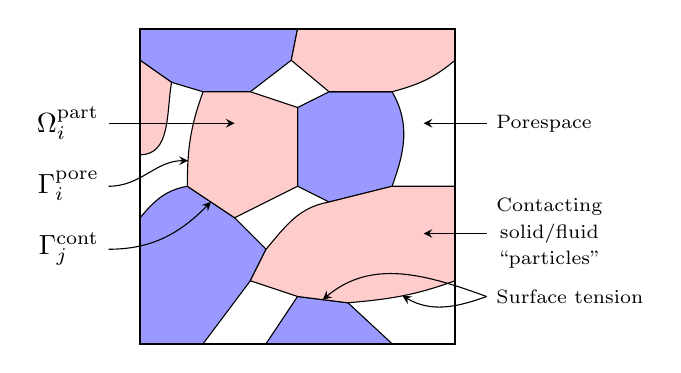
\begin{tikzpicture}[>=stealth,scale=4]
  \coordinate (A) at (0.35,0.2);
  \coordinate (B) at (0.4,0.3);
  \coordinate (C) at (0.3,0.4);
  \coordinate (D) at (0.15,0.5);
  \coordinate (E) at (0.66,0.13);
  \coordinate (F) at (0.6,0.45);
  \coordinate (G) at (0.8,0.5);
  \coordinate (H) at (0.5,0.5);
  \coordinate (I) at (0.5,0.75);
  \coordinate (J) at (0.6,0.8);
  \coordinate (K) at (0.8,0.8);
  \coordinate (L) at (0.35,0.8);
  \coordinate (M) at (0.5,1);
  \coordinate (N) at (0,0.9);
  \coordinate (O) at (0.1,0.83);
  \coordinate (P) at (0.5,0.15);
  \coordinate (Q) at (0.48,0.9);
  \coordinate (R) at (0.2,0.8);
  
  % Region 1 particles 
  \draw[fill=blue!40] 
  (0,0) -- (0.2,0) -- (A) -- (B) -- (C) -- (D) to[out=190,in=50] (0,0.4) -- cycle %A
  (0.4,0) -- (P) -- (E) -- (0.8,0) -- cycle %B
  (F) -- (G) to[out=70,in=-60] (K) -- (J) -- (I) -- (H) -- cycle %C
  (M) -- (Q) -- (L) -- (R) -- (O) -- (N) -- (0,1) -- cycle %D
  ;

  % Region 2 particles
  \draw[fill=red!20]
  (0,0.6) to[out=0,in=-100] (O) -- (N) -- cycle %E
  (D) to[out=90,in=-110] coordinate[near start] (surf3) (R) -- (L) -- (I) -- (H) -- (C) -- (D) coordinate[midway] (surf4) %F
  (M) -- (Q) -- (J) -- (K) to[out=15,in=-140] (1,0.9) -- (1,1) -- cycle %G
  (1,0.2) to[out=-160,in=5] coordinate[midway] (surf1) (E) -- (P) coordinate[midway] (surf2) -- (A) -- (B) to[out=50,in=-170] (F) -- (G) -- (1,0.5) -- cycle %H
  ;

  \draw[thick] (0,0) rectangle (1,1);

  % Annotations
  \draw[<-] (0.9,0.7) -- (1.1,0.7) node[right,font=\scriptsize] {Porespace};
  \draw[<-] (0.9,0.35) -- (1.1,0.35) node[right,font=\scriptsize] {\shortstack{Contacting\\solid/fluid\\``particles''}};
  \draw[<-] (surf1) to[out=-30,in=-160] (1.1,0.15) node[right,font=\scriptsize] {Surface tension};
  \draw[<-] (surf2) to[out=40,in=160] (1.1,0.15); % extra arrow
  \draw[<-] (surf3) to[out=180,in=0] (-0.1,0.5) node[left] {$\Gamma_i^{\mathrm{pore}}$};
  \draw[<-] (surf4) to[out=-135,in=0] (-0.1,0.3) node[left] {$\Gamma_j^{\mathrm{cont}}$};
  \draw[<-] (0.3,0.7) to[out=180,in=0] (-0.1,0.7) node[left] {$\Omega_i^{\mathrm{part}}$};
\end{tikzpicture}
    \includegraphics{sintering_rve.pdf}
    \caption{Microstructure of porous particulate material with sintering particles in contact. The sintering body is subjected to Dirichlet and Neumann boundary conditions on the external boundary.}
    \label{fig:micro}
\end{figure}
%-----------------------------------------------------------------------------


\subsection{Surface tension}

The ``surface tension'' along particle/particle and particle/pore interfaces (the latter denoted pore boundaries) is considered to be the sole ``driving force'' of the sintering process, and it is defined in terms of a ``surface tension force'' acting in the tangent plane of the surface.
In the simplest (and most common) case of isotropic surface tension, this traction is characterized by the constant surface-specific surface energy $\gamma_\surf$ in the current configuration as the single material parameter.
Although we adopt this simplified model below in the numerical results, it is possible to consider the more general situation of anisotropic ``surface stress'' that may also depend on the surface deformation via a suitable constitutive assumption, cf.\ \cite{Steinmann2008:boundaryenergies}.

As shown in, e.g.\ \textsc{\"Ohman et al.} \cite{Ohman2012a}, it is possible to represent the surface tension force by an equivalent surface traction, henceforth denoted $\ta{t}_\fluct$, acting on the surface (or interface).
In the presently assumed case of isotropic surface tension, $\ta{t}_\fluct$ is directed in the normal direction to the surface and is given as
%-----------------------------------------------------------------
\begin{equation}
    \ta{t}_\surf\defeq -\kappa\gamma_\surf\ta{n}
\label{eq:surface_traction_strong}
\end{equation}
%------------------------------------------------------------------
where $\kappa\defeq\ta{n}\cdot\hat{\diff}$ is the curvature.
Here, $\ta{n}$ is taken positive outwards from a convex surface, whereas $\hat\diff \defeq \diff - [\diff\cdot\ta{n}]\ta{n}$ is the surface gradient operator.

\subsection{Incompressible viscous flow of the Stokes' type}

We shall adopt a model for the subscale deformation within the solid particles undergoing the time-dependent sintering process.
The model is simplified in the sense that elastic deformation is neglected a priori.
\todo{REV} This is a common and reasonable simplification for free sintering since the plastic deformation is dominant.
It is then possible to consider a viscoplastic (fluid-like) material with intrinsic incompressibility (within the particles).
Such incompressibility is expressed as $\ta{v}\cdot\ts{\nabla}=0$ and, hence, $\ts{d}_\dev=\ts{d}\defeq[\ta v\outerp\diff]^\sym$.
An isotropic and associated viscoplastic flow rule of the classical Perzyna type is proposed as follows:
%-----------------------------------------------------------------
\begin{equation}
    \ts{d}_\dev = \frac{1}{2\mu}\ts{\sigma}_\dev + \ts{d}_\dev^\pl(\ts{\sigma}_\dev), \quad
    \ts{d}_\dev^\pl = \frac{1}{t_*}\eta\left(\Phi\left(\sigma_\eqv\right)\right)\od{\Phi}{\ts\sigma}
\label{eq:d_sigma}
\end{equation}
%------------------------------------------------------------------
where $t_*$ is the relaxation time, $\eta(\Phi)$ is an overstress function, $\Phi(\sigma_\eqv)$ is the quasistatic yield function and $\sigma_\eqv=\sqrt{\frac{3}{2}}|\ts{\sigma}_\dev|$ is the equivalent stress.
Upon introducing the abbreviated notation $k=\frac{\eta}{t_*}\od{\Phi}{\sigma_\eqv}$, we may solve for $\sigma_\eqv$ in terms of the equivalent rate of deformation $d_\eqv\defeq\sqrt{\frac{2}{3}}|\ts{d}_\dev|$ from the equation
%-----------------------------------------------------------------
\begin{equation}
    \frac{1}{3\mu}\sigma_\eqv + k\left(\sigma_\eqv\right) = d_\eqv
\label{eq:de_sigmae}
\end{equation}
%------------------------------------------------------------------
and we, finally, obtain the ``Newtonian-like'' constitutive relation
%-----------------------------------------------------------------
\begin{equation}
    \ts{\sigma}_\dev(\ts{d}) = 2\tilde{\mu}\ts{d}_\dev, \quad
    \tilde{\mu}\defeq \frac{\sigma_\eqv}{3d_\eqv}
    %\frac{\mu}{1+\frac{3\mu k\left(\sigma_\eqv\left(d_\eqv\right)\right)}{\sigma_\eqv\left(d_\eqv\right)}}
\label{eq:sigma_d}
\end{equation}
%------------------------------------------------------------------

The corresponding tangent stiffness $\tf{E}_{\tang,\dev}$ in the relation $\dif\ts{\sigma}_\dev=\tf{E}_{\tang,\dev}\dprod\dif\ts{d}$ (representing the linearization of the subscale constitutive problem), is given as follows:
%------------------------------------------------------------------
\begin{align}
 \label{eq:E_tang_dev}
 \tf E_{\tang,\dev} &= 2\tilde{\mu} \tf I_\dev + \frac{4}{9 d_\eqv^2} \left[ d_\eqv \left[ \frac{1}{3\mu} + k' \right]^{-1} - \sigma_\eqv \right] \ts d_\dev \outerp\ts d_\dev\\
\intertext{with}
 k' &= \frac{1}{t_*}\left[\eta \frac{\mathrm{d}^2\;\Phi}{\dif\sigma_\eqv^2} + \od{\eta}{\Phi}\left[\od{\Phi}{\sigma_\eqv}\right]^2\right].
\end{align}
%------------------------------------------------------------------

\subsection{Balance equations - Strong and weak formats}
Referring to \figref{fig:micro}, we consider an arbitrarily chosen collection of particles in contact (inside $\Omega$) that constitutes the ``solid particle skeleton''.
Each particle domain $\Omega_i^\particle$ has part of its boundary associated with the pore surface $\Gamma_i^\pore$.
We assume (for simplicity) that the surface tension along the contact surfaces can be ignored. We also introduce the notation $\Omega^\particle \defeq\cup_i\Omega_i^\particle$ and $\Gamma^\pore \defeq \cup_i\Gamma^\pore_i$.

In the absence of acceleration, the balance equations for the quasi-static motion of the assembly of viscoplastic particles can be established in the spatial setting as follows:
%-----------------------------------------------------------------
\begin{subequations}\label{eq:strong_form}
\begin{align}
    -\ts{\sigma}\cdot\diff & = \ts{0} \quad \text{ in }\,\Omega^\particle_i\quad i = 1,2,...
\label{eq:strong_form_v}
\\
    \ta{v}\cdot\diff & = 0 \quad \text{ in }\,\Omega^\particle_i
\label{eq:strong_form_p}
\end{align}
\end{subequations}
\todo{REV} As to the boundary conditions, we note the  surface tension acting on the pore boundary
\begin{align}
   \ta t \defeq \ts\sigma\cdot\ta n &= \ta t_\surf \quad \text{ on }\, \Gamma^\pore_i\quad i = 1,2,..
\label{eq:strong_bc} 
\end{align}
%------------------------------------------------------------------
where $\ts{\sigma}(\ts{d})=\ts{\sigma}_\dev(\ts{d}_\dev)-p\ts{I}$ is the total Cauchy stress, and $p$ is the pressure (Lagrangian multiplier corresponding to the incompressibility constraint).
\todo{REV} In addition, there are boundary conditions (of the Dirichlet and Neumann types) on the exterior surface $\partial\Omega^\particle$ of the considered collection of particles. For simplicity of notation, we assume here that these conditions are homogeneous.

%These surfaces, that are internal to the microstructure, are collectively denoted $\Gamma^\internal=\Gamma^\pore\cup\Gamma^\contact$.
The weak form of \eqref{eq:strong_form} then reads:
%-----------------------------------------------------------------
\todo{REV}
\begin{subequations}\label{eq:weak_form}
\begin{align}
    \int_{\Omega^\particle} \ts{\sigma}\dprod[\delta \ta v\outerp\diff] \dif v
    & =
     \int_{\Gamma^\pore} \ta t_\surf \cdot \delta\ta v \dif a =
    -\int_{\Gamma^\pore} \gamma_\surf\left[\delta\ta{v}\cdot\hat{\diff}\right] \dif a
    %\int_{\Gamma^\pore} \ta{t}_\surf \cdot \delta\ta{v} \dif a
\label{eq:weak_form_v} \\
    \int_{\Omega^\particle} \left[\ta{v}\cdot\diff\right] \delta p \dif v
    & =  0
\label{eq:weak_form_p}
\end{align}
\end{subequations}
%------------------------------------------------------------------
for suitable test functions $\delta\ta{v}$ and $\delta p$ that satisfy the appropriate regularity requirements (not further elaborated in this paper).
To obtain the second integral on the RHS of \eqref{eq:weak_form_v}, that represents ``surface tension loading'', the surface divergence theorem was used for any smooth pore surface segment $\Gamma_i^\pore$. It is noted that $\gamma_\surf$ may be inhomogeneous along $\Gamma^\pore$.

\todo{REV} \textbf{Remark:} In the case that the particle/particle interfaces  have significant surface energy, they can be seen as part of $\Gamma^\pore$.
% 
% \todo{REV} \textbf{Remark}: Equation \eqref{eq:weak_form_v} is obtained by using a weak form for the integral that represents ``surface tension loading'':
% %-----------------------------------------------------------------
% \begin{equation}
%     \int_{\Gamma^\pore} \ta t_\surf \cdot \delta\ta v \dif a =
%     -\int_{\Gamma^\pore} \gamma_\surf\left[\delta\ta{v}\cdot\hat{\diff}\right] \dif a
% \label{eq:surface_traction_weak}
% \end{equation}
% %------------------------------------------------------------------
% where the surface divergence theorem was used for any smooth pore surface segment $\Gamma^\pore_i$. $\Box$

\section{Computational homogenization} \label{sec:homogenization}

\subsection{Representative Volume Element}

In a 2D-representation of the mesoscale features, the appropriately chosen RVE is assumed to occupy the bulk volume $\Omega_\Box(t)$
The RVE must obviously contain a sufficient number of particles and pores to qualify as ``representative'' in the classical sense; however, in order to simplify the subsequent conceptual discussion and ``pave the way'' for the subsequent homogenization, we consider a simple arrangement of particles within the RVE.
In the very simplest case, the RVE consists of one single ``unit cell'' containing a single contiguous pore, \todo{REV} which is the situation shown in \figref{fig:4particleRVE}.
Multi-pore RVEs were investigated in our previous paper \cite{Ohman2012a}.

The current ``bulk'' domain of the RVE at a time $t>0$ contains the particles and the pore space, $\Omega_\Box(t)=\Omega^\particle_\Box(t)\cup\Omega_\Box^\pore(t)$, where $\Omega_\Box^\pore(t)$ is the domain currently occupied by the pore, whereas $\Omega_\Box^\particle(t)$ is occupied by the particles. This is shown schematically in \figref{fig:4particle_rve_b}.
%\footnote{Henceforth, when the time argument is dropped, e.g. $\Omega_\Box$, the current configuration is referred to.}.
The external boundary of the RVE is $\partial\Omega_\Box(t)\defeq\Gamma_\Box(t)$.
The initial configuration of the particles within the RVE (before any deformation has taken place) is denoted $\Omega_\Box(0)$, as shown in \figref{fig:4particle_rve_a}.
%It is noted that in 2D, by assumption, the external boundary of the RVE always cuts through the particles and never through the pore space.
The boundaries of the pore-space are collectively denoted $\Gamma_\Box^\pore(t)$. The boundary of the deforming particles currently contained in the RVE is then $\partial\Omega^\particle_\Box(t)=\Gamma_\Box(t)\cup\Gamma_\Box^\pore(t)$.
%-------------------------------------------------------------------------
\begin{figure}[th!]
    \centering
    \subfloat[$t = 0$]{\label{fig:4particle_rve_a}
%       \tikzsetnextfilename{4particle_rve}
%       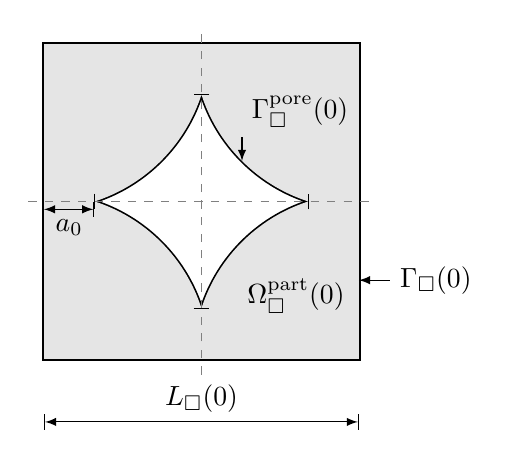
\begin{tikzpicture}[>=latex,scale=2] % Use this to scale the image. Text is always normal-size
  \def\particleradius{1.05} % Adjust this to change the contact size.
  \pgfmathsetmacro{\contactsize}{sqrt(\particleradius^2-1)} % Automatically calculated.
  \begin{scope}[very thick]
  	\draw[clip] (-1,-1) rectangle (1,1);
  	\draw[clip]
  		(-1,-1) circle (\particleradius)
 		( 1,-1) circle (\particleradius)
 		(-1, 1) circle (\particleradius)
   		( 1, 1) circle (\particleradius);
  	\fill[fill=black!10] (-1,-1) rectangle (1,1);
  \end{scope}
  % Markers
  \foreach \q in {0,90,180,270} { \draw[rotate=\q] (1-\contactsize,-0.05) -- +(0,0.1); }
  \draw[dashed,gray] (-1.1,0) -- (1.1,0) (0,-1.1) -- (0,1.1);
  % Annotations
  %\node[below] at (0,0) {$\Omega_\Box^p(0)$};
  \draw[|<->|] (-1,-1.4) -- (1,-1.4) node[midway,above] {$L_\Box(0)$};
  \draw[<->|] (-1,-0.05) -- +(\contactsize,0) node[midway,below] {$a_0$};
  \node at (0.6,-0.6) {$\Omega_\Box^{\mathrm{part}}(0)$};
  \draw[<-] (1,-0.5) -- +(0.2,0) node[right] {$\Gamma_\Box(0)$};
  \draw[<-] (1,1) ++(-135:\particleradius) -- +(0.00,0.15) node[above right] {$\Gamma_\Box^{\mathrm{pore}}(0)$};
  
  %\draw[use as bounding box] (-1.7,-1.5) rectangle (1.7,1.1);
  %\useasboundingbox (-1.7,-1.5) (1.7,1.1);
  % Transformation arrow (makes the picture very unaligned)
  %\draw[->] (1.5,0) to[out=45,in=-150] (2,0);% +(135:0.1) -- (2,0) -- +(-135:0.1);
\end{tikzpicture}

      \includegraphics[width=0.45\linewidth]{4particle_rve.pdf}
    } \hspace{1em}
    \subfloat[$t > 0$]{\label{fig:4particle_rve_b}
%       \tikzsetnextfilename{4particles_deformed}
%       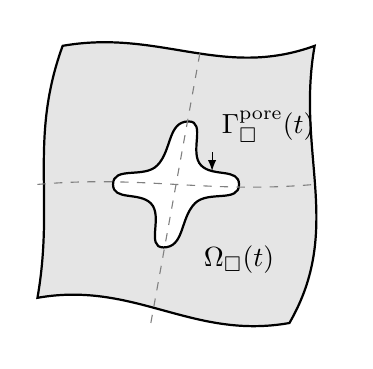
\begin{tikzpicture}[>=latex,scale=1.6] % Use this to scale the image. Text is always normal-size
  \def\particleradius{1.05} % Adjust this to change the contact size.
  \draw[thick,fill=black!10,even odd rule] (0.9,-1.1) 
  	to[out=190,in=10] (-1.1,-0.9)
  	to[out=80,in=-110] (-0.9,1.1)
  	to[out=10,in=-160] (1.1,1.1)
  	to[out=-100,in=60] (0.9,-1.1) -- cycle
  	(-0.1,-0.5) to[out=180,in=-45] (-0.2,-0.15) to[out=135,in=-90]
  	(-0.5,0)    to[out=90,in=-135] (-0.15,0.15)  to[out=45,in=-180]  
  	(0.1,0.5)   to[out=0,in=135]   (0.2,0.15)   to[out=-45,in=90] coordinate[near start] (GammaF)
  	(0.5,0)     to[out=-90,in=45]  (0.15,-0.15)  to[out=-135,in=0] (-0.1,-0.5) -- cycle;
  % Markers
  \draw[dashed,gray] (-1.1,0) to[out=5,in=-175] (1.1,0) (-0.2,-1.1) -- (0.2,1.1);
  % Annotations
  \node at (0.5,-0.6) {$\Omega_\Box(t)$};
  \draw[<-] (GammaF) -- +(0.00,0.15) node[above right] {$\Gamma_\Box^{\mathrm{pore}}(t)$};
\end{tikzpicture}
      \includegraphics[width=0.45\linewidth]{4particles_deformed.pdf}
    }
    \caption{(a) Initial configuration of a single-pore RVE in 2D consisting of circular particles in a perfect square lattice. The contact ``points'' are flattened due to precompaction. (b) Deformed configuration (sketchy).}
    \label{fig:4particleRVE}
\end{figure}
%-----------------------------------------------------------------------------

\subsection{Homogenization -- A format presuming macroscale compressibility}\label{sec:homogencompress}

In the paper by \textsc{\"Ohman et al.} \cite{Ohman2012a} the homogenization theory was presented in a format that is restricted to the situation that the macroscale response is compressible.
In other words, the variational setting for the macroscale problem presumes non-vanishing porespace in the whole macrodomain.
As soon as the porosity reaches zero in any point this format is inadequate and the algorithm breaks down, which is obviously a serious flaw.
The present paper deals with this problem,
\todo{REV}
and the main purpose is to show that it can be alleviated upon introducing a mixed velocity-pressure control on the macro-level.
It is, therefore, relevant to first briefly summarize the theory presented in \cite{Ohman2012a}:

In the most basic format it is only $\ta v$ that is partioned into a smooth (macroscale) part, denoted $\ta{v}^\macro$, and a fluctuating (subscale) part, denoted $\ta{v}^\fluct$. In accordance with the classical assumption of first order homogenization, $\ta{v}^\macro$ is assumed to vary linearly within the RVE, i.e.
%----------------------------------------------------------------------------
\begin{equation}
  \ta{v}^\macro(\bar{\ta{x}};\ta x) = \bar{\ts d}(\bar{\ta x}) \cdot [\ta{x}-\bar{\ta x}] \text{ for }\ta{x}\in\Omega_{\Box}
\label{eq:vm_prolongation}
\end{equation}
%----------------------------------------------------------------------------
or, equivalently
\begin{equation}
 \ta{v}^\fluct = \ta 0 \text{ for }\ta{x}\in\Omega_{\Box}
\label{eq:vm_prolongation_alt}
\end{equation}
i.e. a conventional Dirichlet type boundary condition on the RVEs for the momentum balance equation. \todo{REV}

%----------------------------------------------------------------------------
The link between $\bar{\ta v}$ and $\ta v^\macro$ is established via the macroscale rate-of-deformation tensor $\bar{\ts d}$, defined as
$\bar{\ts d}(\bar{\ta x})\defeq [\bar{\ta v}\outerp \diff]^\sym|_{\bar{\ta x}}$, where $\bar{\ta v}$ is the macroscale velocity field.

As a direct consequence of the assumption that it is only $\ta v$ that is that is prolonged from the macro- to the subscale, it is only the momentum balance that is relevant as a macroscale balance equation. Find $\bar{\ta v} \in \bar{\set{V}}$ that is the solution of
%---------------------------------------------------------------------------------------------------
\begin{align}
 \label{eq:macro_problem_old} \int_\Omega \bar{\ts\sigma}\{\bar{\ts d}\} \dprod [\delta\bar{\ta v}\outerp \diff] \dif v = 0 \quad \forall \delta\bar{\ta v}\in \bar{\set{V}}^0.
\end{align}
%-----------------------------------------------------------------------------------------------------------
where the macroscale (homogenized) stress $\bar{\ts\sigma}$ is computed as
%-----------------------------------------------------------------
\begin{align}
\bar{\ts\sigma} &= 
\langle \ts{\sigma} \rangle_{\Box} -
\frac{1}{|\Omega_{\Box}|}\int_{\Gamma_{\Box}^\pore} [\ts{t}_\surf\otimes[\ts{x}-\bar{\ts{x}}]]^\sym \dif a 
  \\ &= % Broken for 2 column
  \frac{1}{|\Omega_{\Box}|}\int_{\Gamma_{\Box}} [\ts{t}\otimes[\ts{x}-\bar{\ts{x}}]]^\sym \dif a.
\label{eq:sigmmabardef}
\end{align}
%------------------------------------------------------------------
The volume average is defined as
%-------------------------------------------------------------------------------------------
\begin{align}
 \homogenized{[\bullet]}_{\Box}&\defeq\frac{1}{|\Omega_{\Box}|}\int_{\Omega^\particle_{\Box}}[\bullet] \, \dif v,
\end{align}
%----------------------------------------------------------------------------------------------
and it must be noted that, although stresses are defined in the fluid region $\Omega^\particle_{\Box}$, averaging is on the bulk volume $\Omega_{\Box}$.

The RVE-problem is formulated as follows: For given value of the macroscale variable $\bar{\ts d}$, find ($\ta{v}^\fluct,p)\in\set{V}_\Box^{(\Dirichlet)}\times\set{P}_\Box$ that solve the system
%----------------------------------------------------------------------------
\begin{subequations}\label{eq:rve_problem_old}
\begin{alignat}{4}
    & a_\Box(\ta{v}^\macro + \ta{v}^\fluct;\delta \ta{v}^\fluct) +  b_\Box(p,\delta\ta{v}^\fluct)
    && =
    l^\pore_\Box(\delta \ta{v}^\fluct)
    &\;\;& \forall\; \delta \ta{v}^\fluct &&\in \set{V}_\Box^{(\Dirichlet)}
\label{eq:rve_problem_old_v}
 \\
    &b_\Box(\delta p, \ta{v}^\macro+\ta{v}^\fluct)
    && =
    0
    && \forall\; \delta p &&\in \set{P}_\Box
\label{eq:rve_problem_old_p}
\end{alignat}
\end{subequations}
%----------------------------------------------------------------------------
where the variational forms are defined as
%-------------------------------------------------------------------------------
\begin{subequations}\label{eq:subscale_varforms}
\begin{align}
    a_{\Box}(\ta{v};\delta \ta{v}) & \defeq
    \homogenized{ \ts{\sigma}_\dev(\ts{d}) \dprod [\delta\ta v\outerp\diff]}_{\Box} 
    \nonumber\\& = % Broken for 2 column
    \frac{1}{|\Omega_{\Box}|}\int_{\Omega^\particle_{\Box}} \ts{\sigma}_\dev(\ts{d}) \dprod \left[\delta \ta{v}\outerp\diff\right] \dif v
\label{eq:subscale_varforms_a}
\\
    b_{\Box}(p, \delta\ta{v}) & \defeq
    - \homogenized{[\delta\ta{v}\cdot\diff]\; p }_{\Box}
    \nonumber\\ & = % Broken for 2 column
    - \frac{1}{|\Omega_{\Box}|}\int_{\Omega^\particle_{\Box}} [\delta\ta{v}\cdot\diff]\;p \dif v
\label{eq:subscale_varforms_b}
\\
    l_{\Box}^\pore(\delta \ta{v}) & \defeq
    %-\frac{1}{|\Omega_{\Box}|} \int_{\Gamma_{\Box}^\pore} \hat{\ts\sigma}\dprod\left[\delta\ta{v}\outerp\hat{\diff}\right] \dif a
    %\nonumber\\ & = % Broken for 2 column
    -\frac{1}{|\Omega_{\Box}|} \int_{\Gamma_{\Box}^\pore} \gamma_\surf\left[\delta\ta{v}\cdot\hat{\diff}\right] \dif a
\label{eq:subscale_varforms_l}
\end{align}
\end{subequations}
%-----------------------------------------------------------------------------------------
Details regarding the solution of this system in terms of the relevant iteration procedure and how to compute the ATS-tensor in the FE\textsuperscript{2} algorithm are given in \cite{Ohman2012a} and are not further elaborated here. The flow chart is summarized in \figref{fig:box1}.
%-------------------------------------------------------------------------------------------------------------
% \begin{center}
% \fbox{\begin{minipage}{0.98\linewidth}
% BOX1: Summary of FE\textsuperscript{2} format valid only for macroscopic compressibility
% \begin{itemize}
%  \item Macroscale-problem
%  \begin{itemize}
%   \item Fields: $\bar{\ta v}$, solved from \eqref{eq:macro_problem_old}
%  \end{itemize}
%  \item RVE-problem: $\bar{\ts d}_\dev, \bar{e} \longrightarrow \bar{\ts\sigma}_\dev, \bar{p}$
%  \begin{itemize}
%   \item Input: $\bar{\ts d}$ (or $\bar{\ts d}_\dev, \bar{e}$)
%   \item Fields: $\ta v^\fluct$, $p$, solved from \eqref{eq:rve_problem_old}
%   \item Output: $\bar{\ts\sigma}$ (post-processed) $\longrightarrow \bar{\ts\sigma}_\dev, \bar{p}$
%  \end{itemize}
% \end{itemize}
% \end{minipage}}
% \end{center}
\begin{figure}
 \centering
%  \tikzsetnextfilename{box1}
%  \begin{tikzpicture}[node distance = 2cm, auto,scale=0.8, transform shape, >=latex']
    %\small
    %\tikzstyle{every node}=[font=\footnotesize]
    \tikzstyle{group}    = [rectangle, draw, thick, dashed, text width=6em, text centered, rounded corners]
    \tikzstyle{decision} = [diamond,   draw, fill=white, aspect=2, node distance=2.5cm, inner sep=2pt]
    \tikzstyle{block}    = [rectangle, draw, fill=white, text width=6em, text centered, rounded corners]
    \tikzstyle{line}     = [draw, ->]

    \draw [thick, dashed, fill=blue!10, rounded corners] (-4.5,0.5) rectangle ( 1.9,-7.8);
    \draw [thick, dashed, fill=red!10,  rounded corners] ( 3.8,0.5) rectangle (10.1,-7.8);
    \node [below right, inner sep=10pt] at (-4.5,0.5) { \textbf{\large Macro} };
    \node [below left,  inner sep=10pt] at (10.1,0.5) { \textbf{\large RVE} };

    % Place nodes
    \node [block] (init) {Initial guess};
    \node [block, below of=init, text width=8em, node distance=1.5cm] (residual) {Compute residual from (12)};
    \node [decision, below of=residual,node distance=2cm] (convergence) {Converged?};
    \node [block, below of=convergence, node distance=2.3cm] (stop) {Finish step};
    \node [block, left of=stop, node distance=3cm] (update) {Newton iteration: Compute tangent};
    % Draw edges
    \path [line] (init) -- (residual) node[midway] {$\bar{\ta{v}}$};
    \path [line] (residual) -- (convergence);
    \path [line] (convergence) -- node {False} (update);
    \path [line] (convergence) -- node {True} (stop);
    \path [line] (update) |- node[near start,right] {$\bar{\ta{v}}$} (residual);

    % Place nodes
    \node [block, right of=init, node distance=5.6cm] (rve_init) {Initial guess};
    \node [block, below of=rve_init, text width=8em, node distance=1.5cm] (rve_residual) {Compute residual from (16)};
    \node [decision, below of=rve_residual, node distance=2cm] (rve_convergence) {Converged?};
    \node [block, below of=rve_convergence, node distance=2.3cm] (rve_stop) {Post-process $\bar{\ts\sigma}$};
    \node [block, right of=rve_stop, node distance=3cm] (rve_update) {Newton iteration: Compute tangent};
    % Sensitivity problem
    \node [block, below of=rve_stop, node distance=1.3cm] (rve_sensitivity) {Sensitivity problem};
    
    % Draw edges
    \path [line] (rve_init) -- (rve_residual) node[midway] {$\ta{v}^\fluct,p$};
    \path [line] (rve_residual) -- (rve_convergence);
    \path [line] (rve_convergence) -- node {False} (rve_update);
    \path [line] (rve_convergence) -- node {True} (rve_stop);
    \path [line] (rve_update) |- node[right, near start] {$\ta{v}^\fluct,p$} (rve_residual);

    \path [line] (residual.east) ++(0, 0.2cm) -- ++(0.7cm,0) |- node [below,pos=0.65] {$\bar{\ts d}_\dev, \bar{e}$} (rve_init);
    % Draw this backwards in order to get exact alignments
    \path [line, <-] (residual.east) ++(0,-0.2cm) -- ++(0.7cm,0) |- node [below,pos=0.65] {$\bar{\ts\sigma}_\dev, \bar{p}$} (rve_stop);

    \path [line] (rve_sensitivity) -| node[below, pos=0.10] {$\bar{\tf E}$} (update);
\end{tikzpicture}

 \includegraphics{box1.pdf}
 \caption{Flow-chart of FE\textsuperscript{2}-format valid only for macroscopic compressibility}
 \label{fig:box1}
\end{figure}

%---------------------------------------------------------------------------------------------------------
In \figref{fig:box1}, we used the split into deviatoric and volumetric parts:
%------------------------------------------------------------------------------------------------------------
\begin{alignat}{3}
    &\bar{\ts d} = \bar{\ts d}_\dev + \frac{1}{3}\bar{e} \ts I
    &\;\;&\text{where}\;\; \bar{e} \defeq \bar{\ts d}\dprod \ts I,&\;\;& \bar{\ts d}_\dev \defeq \bar{\ts d} - \frac13\bar{e}\ts I \\
    &\bar{\ts\sigma} = \bar{\ts\sigma}_\dev - \bar{p} \ts I
    &\;\;&\text{where}\;\; \bar{p} \defeq -\frac13 \bar{\ts\sigma}\dprod \ts I,&\;\;& \bar{\ts\sigma}_\dev \defeq \bar{\ts\sigma} + \bar{p} \ts I
\end{alignat}
%-------------------------------------------------------------------------------------------------------------------
and where $\bar{\ts d}_\dev = [\bar{\ta v} \outerp\diff]^\sym_\dev$, $\bar{e} = \bar{\ta v}\cdot\diff$.

\textbf{Remark}: The split in deviatoric and volumetric parts is never (or at least does not need to be) exploited operationally in the numerical algorithm; however, the situation is entirely different in the format discussed in the next Section. $\Box$

\subsection{Homogenization -- A format allowing transition from macroscale compressibility to incompressibility}\label{sec:homogencompressincompress }

In this Section we outline the strategy for replacing the velocity-based format in Section \ref{sec:homogencompress} to a mixed variational format on the macroscale.
Hence, we introduce the macroscale pressure $\bar{p}$ as an independent variable in the momentum balance equation, and the relation $\bar{e} = \bar{\ta v}\cdot\diff$ is imposed in a weak sense.
The resulting macroscale problem then becomes: Find $(\bar{\ta v},\bar{p}) \in \bar{\set{V}}\times\bar{\set{P}}$ that solve
%-------------------------------------------------------------------------------------------------------------------------------------
\begin{subequations}\label{eq:macro_problem_new}
\begin{alignat}{3}
 &\int_\Omega \bar{\ts\sigma}_\dev\{\bar{\ts d}_\dev,\bar{p}\} \dprod [\delta\bar{\ta v}\outerp \diff] \dif v + \int_\Omega -\bar{p}\;[\delta\bar{\ta v}\cdot\diff]\dif v &&= 0 &\quad& \forall \delta\bar{\ta v}\in \bar{\set{V}}^0\\
 &\int_\Omega \left[\bar{e}\{\bar{\ts d}_\dev,\bar{p}\} - \bar{\ta v}\cdot\diff\right]\delta\bar{p} \dif v &&= 0&\quad& \forall \delta\bar{p}\in \bar{\set{P}}
\end{alignat}
\end{subequations}
%----------------------------------------------------------------------------------------------------------------------------------------
which system of equations thus replaces (\ref{eq:macro_problem_old}).

The prolongation of $\bar{\ts d}$ to the RVE remains as before; however, it is useful to note that $\ta{v}^\macro$ can be expanded as
%----------------------------------------------------------------------------------------------------------------------------------------
\begin{align}
\ta{v}^\macro = \ta{v}^\macro_\dev + \ta{v}^\macro_\vol = \bar{\ts d}_\dev\cdot [\ta x-\bar{\ta x}]+ \bar{e} \frac13 [\ta x - \bar{\ta x}]
\end{align}
%----------------------------------------------------------------------------------------------------------------------------------------

The important difference to the previous formulation is that the volumetric part is no longer an input but part of the solution of the RVE-problem.
The corresponding complementary equation is obtained upon testing the momentum balance equation with the volumetric part of $\ta{v}^\macro$.
As the result, we obtain the following RVE-problem: For given macroscale variables $\bar{\ts d}_\dev$ and $\bar{p}$, find  ($\ta{v}^\fluct,p,\bar{e})\in\set{V}_\Box^{(\Dirichlet)}\times\set{P}_\Box\times\set{R}$ that solve the system
%----------------------------------------------------------------------------
\begin{subequations}\label{eq:rve_problem_new}
\begin{alignat}{4}
    & a_\Box(\ta{v}^\macro_\dev(\bar{\ts d}_\dev) + \ta{v}^\fluct;\delta \ta{v}^\fluct) +  b_\Box(p,\delta\ta{v}^\fluct)
    && =
    l^\pore_\Box(\delta \ta{v}^\fluct)
    &\;\;& \forall\; \delta \ta{v}^\fluct &&\in \set{V}_\Box^{(\Dirichlet)}
\label{eq:rve_problem_new_v}
 \\
    &b_\Box(\delta p, \ta{v}^\macro_\vol(\bar{e})+\ta{v}^\fluct)
    && =
    0
    && \forall\; \delta p &&\in \set{P}_\Box
\label{eq:rve_problem_new_p}
\\
    &b_\Box(p,\ta{x}_\mean)\delta\bar{e}
    && =
    [l_\Box^\pore(\ta{x}_\mean) - \bar{p}]\delta\bar{e}
    && \forall\; \delta\bar{e} &&\in \set{R}
\label{eq:rve_problem_new_d}
\end{alignat}
\end{subequations}
%%----------------------------------------------------------------------------
where $\ta{x}_\mean \defeq \frac13[\ta x-\bar{\ta x}]$. \todo{REV} Detailed derivations of \eqref{eq:rve_problem_new_v} and \eqref{eq:rve_problem_new_d} are shown in \ref{appendix:RVE}.

\todo{REV} It is worth noting that the space of test functions for the subscale fluctuation fields, $\set{V}_\Box^{(\Dirichlet)}$, have not changed in this new formulation, and $\ta v^\fluct$ is still zero on the RVE boundary.
Hence, Dirichlet boundary conditions are still adopted for the velocity field.
Only the control variables, summarized in \figref{fig:box2}, have changed.

\todo{REV} It turns out that the physical interpretation of \eqref{eq:rve_problem_new_d} is that the RVE pressure plus the surface tension contribution must equal the macroscopic pressure;
\begin{align}
 \homogenized{p}_\Box + \frac{1}{|\Omega_\Box|} \int_{\Gamma_\Box^\pore} \frac23 \gamma_\surf\dif A= \bar{p}.
\end{align}


As to the ``feed-back'' of variables to the macroscale problem, we note that that $\bar{e}$ is part of the solution of the RVE-problem, whereas $\bar{\ts\sigma}_{\dev}\{\bar{\ts d}_\dev,\bar{p}\}$ is post-processed as
%-----------------------------------------------------------------------------------------------------
\begin{align}\label{eq:sigma_bar_dev_hom}
 \bar{\ts\sigma}_\dev = \frac{1}{|\Omega_\Box|}\int_{\Gamma_\Box} [\ta t \outerp [\ta x-\bar{\ta x}]]^\sym \dif a + \bar{p}\ts I
\end{align}
%----------------------------------------------------------------------------------
\textbf{Remark}: It was used explicitly in \eqref{eq:rve_problem_new_v} that $\ta{\sigma}_\dev$ is proportional to ${\ts d}_\dev$. $\Box$
%----------------------------------------------------------------------------------------------------------------
% \begin{center}
% \fbox{\begin{minipage}{0.98\linewidth}
% BOX2 Summary of FE\textsuperscript{2} format for seamless transition from macroscopic compressibility to incompressibility
% \begin{itemize}
%  \item Macroscale-problem
%  \begin{itemize}
%   \item Fields: $\bar{\ta v}$, $\bar{p}$, solved from  \eqref{eq:macro_problem_new}
%   \item Constitutive behavior: At every integration point, evaluate $\bar{\ts d}_\dev$, $\bar{p}$ and solve the RVE problem
%  \end{itemize}
%  \item RVE-problem: $\bar{\ts d}_\dev, \bar{p} \longrightarrow \bar{\ts\sigma}_\dev, \bar{e}$
%  \begin{itemize}
%   \item Input: $\bar{\ts d}_\dev$, $\bar{p}$
%   \item Fields: $\ta v^\fluct$, $p$, $\bar{e}$, solved from \eqref{eq:rve_problem_new}
%   \item Output: $\bar{\ts\sigma}_\dev$ (post-processed), $\bar{e}$
%  \end{itemize}
% \end{itemize}
% \end{minipage}}
% \end{center}
\begin{figure}
 \centering
%  \tikzsetnextfilename{box2}
%  \begin{tikzpicture}[node distance = 2cm, auto,scale=0.8, transform shape, >=latex']
    %\small
    %\tikzstyle{every node}=[font=\footnotesize]
    \tikzstyle{group}    = [rectangle, draw, thick, dashed, text width=6em, text centered, rounded corners]
    \tikzstyle{decision} = [diamond,   draw, fill=white, text width=6em, text centered, aspect=2, node distance=2.5cm, inner sep=2pt]
    \tikzstyle{block}    = [rectangle, draw, fill=white, text width=6em, text centered, rounded corners]
    \tikzstyle{line}     = [draw, ->]

    \draw [thick, dashed, fill=blue!10, rounded corners] (-4.5,0.5) rectangle ( 1.9,-7.8);
    \draw [thick, dashed, fill=red!10,  rounded corners] ( 3.8,0.5) rectangle (10.1,-7.8);
    \node [below right, inner sep=10pt] at (-4.5,0.5) { \textbf{\large Macro} };
    \node [below left,  inner sep=10pt] at (10.1,0.5) { \textbf{\large RVE} };

    % Place nodes
    \node [block] (init) {Initial guess};
    \node [block, below of=init, text width=8em, node distance=1.5cm] (residual) {Compute residual from (20)};
    \node [decision, below of=residual,node distance=2cm] (convergence) {Converged?};
    \node [block, below of=convergence, node distance=2.3cm] (stop) {Finish step};
    \node [block, left of=stop, node distance=3cm] (update) {Newton iteration: Compute tangent};
    % Draw edges
    \path [line] (init) -- (residual) node[midway] {$\bar{\ta{v}},\bar{p}$};
    \path [line] (residual) -- (convergence);
    \path [line] (convergence) -- node {False} (update);
    \path [line] (convergence) -- node {True} (stop);
    \path [line] (update) |- node[near start,right] {$\bar{\ta{v}},\bar{p}$} (residual);

    % Place nodes
    \node [block, right of=init, node distance=5.6cm] (rve_init) {Initial guess};
    \node [block, below of=rve_init, text width=8em, node distance=1.5cm] (rve_residual) {Compute residual from (22)};
    \node [decision, below of=rve_residual, node distance=2cm] (rve_convergence) {Converged?};
    \node [block, below of=rve_convergence, node distance=2.3cm] (rve_stop) {Post-process $\bar{\ts\sigma}_\dev$};
    \node [block, right of=rve_stop, node distance=3cm] (rve_update) {Newton iteration: Compute tangent};
    % Sensitivity problem
    \node [block, below of=rve_stop, node distance=1.3cm] (rve_sensitivity) {Sensitivity problem (36)};
    
    % Draw edges
    \path [line] (rve_init) -- (rve_residual) node[midway] {$\ta{v}^\fluct,p, \bar{e}, \ta t, \bar{\ts\sigma}_\dev$};
    \path [line] (rve_residual) -- (rve_convergence);
    \path [line] (rve_convergence) -- node {False} (rve_update);
    \path [line] (rve_convergence) -- node {True} (rve_stop);
    \path [line] (rve_update) |- node[right, near start, text width=1.5em] {$\ta{v}^\fluct,p$, $\bar{e}, \ta t, \bar{\ts\sigma}_\dev$} (rve_residual);

    \path [line] (residual.east) ++(0, 0.2cm) -- ++(0.7cm,0) |- node [below,pos=0.65] {$\bar{\ts d}_\dev, \bar{p}$} (rve_init);
    % Draw this backwards in order to get exact alignments
    \path [line, <-] (residual.east) ++(0,-0.2cm) -- ++(0.7cm,0) |- node [below,pos=0.65] {$\bar{\ts\sigma}_\dev, \bar{e}$} (rve_stop);

    \path [line] (rve_sensitivity) -| node[below, pos=0.10] {$\substack{\displaystyle\bar{\tf E}_\ded,\bar{\ts C}_\ded \\ \displaystyle\bar{\ts E}_\dep,\bar{C}_\dep}$} (update);
\end{tikzpicture}

 \includegraphics{box2.pdf}
 \caption{Flow-chart of FE\textsuperscript{2}-format for seamless transition from macroscopic compressibility to incompressibility}
 \label{fig:box2}
\end{figure}
%-------------------------------------------------------------------------------------------------------------------------------
\subsubsection*{Macroscale incompressibility}
Consider the extreme situation of macroscopic incompressibility, defined by the condition $\bar{e}=0$. The system \eqref{eq:macro_problem_new} is then simplified as follows:
%-------------------------------------------------------------------------------------------------------------------------------------
\begin{subequations}\label{eq:macro_problem_new_incomp}
\begin{alignat}{2}
 &\int_\Omega \bar{\ts\sigma}_\dev\{\bar{\ts d}_\dev,\bar{p}\} \dprod [\delta\bar{\ta v}\outerp \diff] \dif v + \int_\Omega -\bar{p}\;[\delta\bar{\ta v}\cdot\diff]\dif v = 0 &\quad& \forall \delta\bar{\ta v}\in \bar{\set{V}}^0\\
 &\int_\Omega \bar{\ta v}\cdot\diff\delta\bar{p} \dif v &\quad& \forall \delta\bar{p}\in \bar{\set{P}}
\end{alignat}
\end{subequations}
%----------------------------------------------------------------------------------------------------------------------------------------
i. e. $\bar{p}$ is now a classical Lagrange multiplier. Moreover, the result $\bar{e}=0$ is obtained as part of the solution of the simplified RVE-problem \eqref{eq:rve_problem_new} from setting  $l^\pore_\Box(\delta \ta{v}^\fluct)=0$:
%----------------------------------------------------------------------------
\begin{subequations}\label{eq:rve_problem_new_incomp}
\begin{alignat}{4}
    & a_\Box(\ta{v}^\macro_\dev(\bar{\ts d}_\dev) + \ta{v}^\fluct;\delta \ta{v}^\fluct) +  b_\Box(p,\delta\ta{v}^\fluct)
    && =
    0
    &\quad& \forall\; \delta \ta{v}^\fluct &&\in \set{V}_\Box^{(\Dirichlet)}
\label{eq:rve_problem_new_v_incomp}
 \\
    &b_\Box(\delta p, \ta{v}^\macro_\vol(\bar{e})+\ta{v}^\fluct)
    && =
    0
    && \forall\; \delta p &&\in \set{P}_\Box
\label{eq:rve_problem_new_p_incomp}
\\
    &b_\Box(p,\ta{x}_\mean)\delta\bar{e}
    && =
    - \bar{p}\delta\bar{e}
    && \forall\; \delta\bar{e} &&\in \set{R}
\label{eq:rve_problem_new_d_incomp}
\end{alignat}
\end{subequations}

\todo{REV} More precisely, $\bar{e} = 0$ is obtained as the solution of \eqref{eq:rve_problem_new_p_incomp} upon choosing $\delta p = 1$.
Furthermore \eqref{eq:rve_problem_new_d_incomp} guarantees a unique solution $\ta v^\fluct$, $p$ for the incompressible Stokes' problem by omitting the otherwise arbitrary constant in $p$.

%%----------------------------------------------------------------------------
We thus remark that the problem format employed in (\ref{eq:macro_problem_new}) does indeed represent both the macroscopically compressible and incompressible states such that the transition between them is seamless.
% ----------------------------------------------------------------------------
\subsection{Iterative solution of RVE-problem using Newton's method}

The RVE-problem \eqref{eq:rve_problem_new} must be solved iteratively in practice due to the subscale nonlinearities.
To this end, we first rewrite the RVE-problem as the vanishing residuals
%----------------------------------------------------------------------------
\begin{subequations}
\begin{alignat}{4}
  &R_\Box^\derv(\ta{v}^\fluct,p; \delta \ta{v}^\fluct)
  &&\defeq l_\Box^\pore(\delta \ta{v}^\fluct) -
    a_\Box(\ta{v}^\macro_\dev(\bar{\ta{d}}_\dev)+\ta{v}^\fluct;\delta \ta{v}^\fluct) -
    b_\Box(p,\delta\ta{v}^\fluct)
  &\quad& \forall\; \delta \ta{v}^\fluct &&\in \set{V}_\Box^{(\Dirichlet)}
  \\
  &R_\Box^\dep(\bar{e},\ta{v}^\fluct; \delta p)
  &&\defeq - b_\Box(\delta p,\ta{v}^\macro_\vol(\bar{e})+\ta{v}^\fluct)
  && \forall\; \delta p &&\in \set{P}_\Box
  \\
  &R_\Box^\ded(p;\delta\bar{e})
  &&\defeq [l_\Box^\pore(\ta{x}_\mean) - \bar{p} - b_\Box(p,\ta{x}_\mean)]\delta\bar{e}
  && \forall\; \delta\bar{e} &&\in \set{R}
\end{alignat}
\end{subequations}
%----------------------------------------------------------------------------
Newton's iteration method for finding the unknown variables
$\ta{v}^\fluct, p, \bar{e}$ for given $\bar{\ts d}_\dev$ and $\bar{p}$ then becomes: For $k=1,2,\ldots,$ compute
%----------------------------------------------------------------------------
\begin{equation}
    {\ta{v}}^{\fluct(k+1)} = {\ta{v}}^{\fluct(k)} + \Delta {\ta{v}}^\fluct, \quad
    p^{(k+1)} = p^{(k)} + \Delta p, \quad
    \bar{e}^{(k+1)} = \bar{e}^{(k)} + \Delta \bar{e}
\label{eq251}
\end{equation}
%----------------------------------------------------------------------------
where the iterative updates $\Delta {\ta{v}}^\fluct\in{\set{V}}_\Box^{(\Dirichlet)}, \Delta p \in{\set{P}}_\Box, \Delta\bar{e}\in\set{R}$ are solved from the tangent equations
%----------------------------------------------------------------------------
\begin{subequations}\label{eq:rve_iterative}
\begin{alignat}{4}
    &(a_\Box)'(\ta v^\macro_\dev + \ta v^{\fluct(k)}; \delta\ta{v}^\fluct,\Delta \ta{v}^\fluct)
    + b_\Box(\Delta p,\delta\ta{v}^\fluct)
    && = R_\Box^\derv(\bullet^{(k)}; \delta\ta{v}^\fluct)
    &\quad& \forall\; \delta \ta{v}^\fluct &&\in \set{V}_\Box^{(\Dirichlet)}
    \\
    &b_\Box(\delta p,\ta{v}^\macro_\vol(\Delta\bar{e}) + \Delta\ta{v}^\fluct)
    && = R_\Box^\dep(\bullet^{(k)}; \delta p)
    && \forall\; \delta p &&\in \set{P}_\Box
    \\
    &b_\Box(\Delta p,\ta{x}_\mean)\delta\bar{e}
    && = R_\Box^\ded(\bullet^{(k)}; \delta\bar{e})
    && \forall\; \delta\bar{e} &&\in \set{R}
\end{alignat}
\end{subequations}
%----------------------------------------------------------------------------
until the residuals are sufficiently small.
The tangent form $(a_\Box)'$ is given explicitly as
%----------------------------------------------------------------------------
\begin{align}
    (a_\Box)'(\bullet; \delta \ta{v}^\fluct,\Delta{\ta{v}}^\fluct)
    & =
    \left\langle \left[\delta\ta{v}\outerp\diff\right] \dprod \tf{E}_{\majorT,\dev}(\bullet) \dprod
    \left[\Delta\ta{v}^\fluct\outerp\diff\right] \right\rangle_\Box
\end{align}
%----------------------------------------------------------------------------
where the tangent $\tf{E}_{\majorT,\dev}$ is defined in \eqref{eq:E_tang_dev}. \todo{REV}


\section{Mixed macroscale problem format -- Selected issues}

\subsection{Macroscale problem -- Abstract format}

The macroscale problem in \eqref{eq:macro_problem_new} can be put in the more abstract form as follows: Find $(\bar{\ta v},\bar p) \in\bar{\set V}\times\bar{\set{P}}$ that solve
%----------------------------------------------------------------------------
\begin{subequations}\label{eq411}
\begin{alignat}{3}
 &\bar a\{\bar{\ta v},\bar p; \delta\bar{\ta v}\} + \bar b\{\bar p, \delta\bar{\ta v}\} &&= 0   &&\quad \forall\; \delta\bar{\ta v} \in \bar{\set{V}}^0
 \label{eq411a}\\
 &\bar b\{\delta\bar p, \bar{\ta v}\} + \bar c\{\bar{\ta v}, \bar p; \delta\bar p\} &&= 0   &&\quad \forall\; \delta\bar p \in \bar{\set{P}}
 \label{eq411b}
\end{alignat}
\end{subequations}
%----------------------------------------------------------------------------
where the pertinent variational forms are given as
%----------------------------------------------------------------------------
\begin{align}
 \bar a\{\bar{\ta v},\bar p; \delta\bar{\ta v}\} &\defeq \int_\Omega \bar{\ts\sigma}_\dev\{\left[\bar{\ta v}\outerp \diff\right]^\sym_\dev,\bar p\}\dprod \left[\delta\bar{\ta v}\outerp \diff\right]^\sym_\dev \dif v
 \label{eq412a}\\
 \bar b\{\bar p, \delta\bar{\ta v}\}             &\defeq -\int_\Omega \bar p\left[\delta\bar{\ta v}\cdot\diff\right]\dif v
 \label{eq412b}\\
 \bar c\{\bar{\ta v}, \bar p; \delta\bar p\}     &\defeq \int_\Omega \bar{e}\{\left[\bar{\ta v}\outerp \diff\right]^\sym_\dev,\bar p\}\delta\bar p\dif v
 \label{eq412c}
 %\bar l\{\delta\bar {\ta v}\}               &\defeq \int_{\Gamma^\external_\Neumann} \bar{\ta t}_\prescribed\cdot \delta\bar{\ta v} \dif a
 %\label{eq412d}
\end{align}
%----------------------------------------------------------------------------
%In order to motivate the boundary term \eqref{eq412d}, we have assumed sufficient smoothness of the prescribed traction $\bar{\ta t}_\prescribed$.
Newton iterations for solving the system \eqref{eq411} employ the algorithmic tangents
%----------------------------------------------------------------------------
\begin{subequations}\label{eq413}
\begin{align}
 \dif \bar{\ts\sigma}_\dev &= \bar{\tf E}_\ded \dprod \dif\bar{\ts d}_\dev + \bar{\ts E}_\dep \dif\bar{p}
 \label{eq413a} \\
 \dif \bar{e} &= \bar{\ts C}_\ded \dprod \dif \bar{\ts d}_\dev + \bar{C}_\dep \dif\bar{p}
 \label{eq413b}
\end{align}
\end{subequations}
%-----------------------------------------------------------------------------
taken with respect to $\bar{\ts d}_\dev \defeq [\bar{\ta v}\outerp\diff]^\sym_\dev$ and $\bar p$, such that the increments $\Delta\bar{\ta v}$ and $\Delta\bar{p}$ are obtained from the macroscale tangent problem
%----------------------------------------------------------------------------
\begin{subequations}\label{eq:macro_tangent_problem}
\begin{multline}
  \bar{a}'_\derv\{\bullet; \delta\bar{\ta v},\Delta\bar{\ta v}\} + \bar{a}'_\dep\{\bullet; \delta\bar{\ta v},\Delta\bar{p}\} + \bar{b}\{\Delta\bar p, \delta\bar{\ta v}\}
  \\= - \bar{a}\{\bullet; \delta\bar{\ta v}\} - \bar{b}\{\bullet, \delta\bar{\ta v}\}
  \quad\forall\; \delta\bar{\ta v} \in \bar{\set{V}}^0
\label{eq:macro_tangent_problem_v}
\end{multline}
\begin{multline}
  \bar{b}\{\delta\bar p, \Delta\bar{\ta v}\} + \bar{c}'_\derv\{\bullet; \delta\bar{p}, \Delta\bar{ \ta v}\} + \bar{c}'_\dep\{\bullet; \delta\bar{p},\Delta\bar{p}\}
  \\= -\bar{b}\{\delta\bar{p},\bullet\} - \bar{c}\{\bullet;\delta\bar{p}\}
  \quad\;\,\forall\; \delta\bar{p} \in \bar{\set{P}}
\label{eq:macro_tangent_problem_p}
\end{multline}
\end{subequations}
%----------------------------------------------------------------------------
where
%----------------------------------------------------------------------------
\begin{align}
 \bar{a}'_\derv\{\bullet; \delta\bar{\ta v},\Delta\bar{\ta v}\} &= \int_\Omega \left[\delta\bar{\ta v}\outerp\diff\right]^\sym_\dev \dprod \bar{\tf{E}}_\ded \dprod \left[\Delta\bar{\ta v}\outerp\diff\right]^\sym_\dev \dif v
 \label{eq415a}\\
 \bar{a}'_\dep\{\bullet; \delta\bar{\ta v},\Delta\bar{p}\}     &= \int_\Omega \left[\delta\bar{\ta v}\outerp\diff\right]^\sym_\dev \dprod \bar{\ts E}_\dep \,\Delta\bar{p} \dif v
 \label{eq415b}\\
 \bar{c}'_\derv\{\bullet; \delta\bar{p}, \Delta\bar{ \ta v}\}   &= \int_\Omega \delta\bar{p} \,\bar{\ts C}_\ded \dprod \left[\Delta\bar{\ta v}\outerp\diff\right]^\sym_\dev \dif v
 \label{eq415c}\\
 \bar{c}'_\dep\{\bullet; \delta\bar{p},\Delta\bar{p}\}         &= \int_\Omega \delta\bar{p} \,\bar{C}_\dep \Delta\bar p\dif v
 \label{eq415d}
\end{align}
%----------------------------------------------------------------------------
% \textbf{Remark}: In the incompressible case, \eqref{eq411} can be replaced by the classical format
% %----------------------------------------------------------------------------
% \begin{subequations}\label{eq420}
% \begin{alignat}{3}
%  &\bar a\{\bar{\ta v},\bar p; \delta\bar{\ta v}\} + \bar b\{\bar p, \delta\bar{\ta v}\}
%  &&= 0
%  &\quad& \forall\; \delta\bar{\ta v} \in \bar{\set{V}}^0
%  \label{eq420a}\\
%  &\bar b\{\delta\bar p, \bar{\ta v}\}
%  &&= 0
%  &\quad& \forall\; \delta\bar p \in \bar{\set{P}}
%  \label{eq420b}
% \end{alignat}
% \end{subequations}
% %----------------------------------------------------------------------------
% However, \eqref{eq411} is always retained as the operational formulation in practice. $\Box$
% 

%Special issues related to the RVE-problem will be discussed. These are (1) the iterative solution, (2) computation of macroscale algorithmic tangent tensors, (3) symmetry properties of the total macroscale tangent in the mixed format.


\subsection{Computation of macroscale algorithmic tangent tensors}

The algorithmic tensors $\bar{\tf{E}}_\ded, \bar{\ts E }_\dep, \bar{\ts C}_\ded$ and $\bar{C}_\dep$, needed in order to carry out macroscale Newton iterations in \eqref{eq:macro_tangent_problem}, are obtained for perturbations of the RVE-solution expressed in terms of perturbations of $\bar{\ts d}_\dev$ and $\bar{p}$. However, in order to obtain a suitable representation of deviatoric macroscale 2nd order tensors, we conclude that it is convenient to replace the standard dyad bases with a complete, orthonormal, basis $\{\ts E_i\}_{i=1}^{n_{\mathrm{b}}}$ for symmetric deviatoric tensors.
Hence, these base dyadics satisfy the conditions $\ts E_i \dprod \ts E_j = \delta_{ij}$ and $\ts E_i\dprod{\ts I}=0$.
Examples of such bases are shown in the Appendix. We may now adopt the expansions
%----------------------------------------------------------------------------
\begin{align}
 \bar{\ts d}_\dev &= \sum_i^{n_{\mathrm{B}}} \bar{d}_{\dev,i} \ts E_i,\quad  \bar{d}_{\dev,i} = \bar{\ts d}_\dev\dprod \ts E_i
\label{eq:d_dev_base} \\
 \bar{\ts\sigma}_\dev &= \sum_i^{n_{\mathrm{B}}} \bar{\sigma}_{\dev,i} \ts E_i,\quad \bar{\sigma}_{\dev,i} = \bar{\ts\sigma}_\dev\dprod \ts E_i
\label{eq:s_dev_base}
\end{align}
%----------------------------------------------------------------------------
\textbf{Remark}: For 3D $n_{\mathrm{B}} = 5$, while for 2D $n_{\mathrm{B}} = 2$.

We are now in the position to compute \emph{sensitivity fields}, corresponding to a unit variation of the macroscale variables $\bar{d}_{\dev,i}$ and $\bar{p}$. First, we shall need to compute the differentials
%----------------------------------------------------------------------------
\begin{align}
    \dif\ta{v}
     = &
    \dif\ta{v}^\macro_\dev + \dif\ta{v}^\macro_\vol + \dif\ta{v}^\fluct.
\label{eq:dv}
\end{align}
%----------------------------------------------------------------------------------
Using \eqref{eq:d_dev_base} we obtain
%----------------------------------------------------------------------------
\begin{align}
  \dif \ta{v}^{\macro}_\dev &= \sum_{i} \hat{\ta{v}}^{\macro(i)}_\dev \dif\bar{d}_{\dev,i}, \quad  \hat{\ta{v}}^{\macro(i)}_\dev = \ts E_i \cdot [\ta x - \bar{\ta x}]
\label{eq216}
%\dif\ta{v}^\macro_\vol &= \ta x_\mean \dif \bar{e}
\end{align}
%----------------------------------------------------------------------------
where $\hat{\ta{v}}^{\macro(i)}_\dev$ are the ``unit velocity fields''. In analogy with the definition of $\hat{\ta{v}}^{\macro(i)}_\dev$
in \eqref{eq216}, we introduce the ``unit fields'', or sensitivities, due to a unit perturbation of the components $\dif\bar{d}_{\dev,i}$ and of $\dif\bar{p}$, via the \emph{ansatz}
%----------------------------------------------------------------------
\begin{align}
    \dif\ta{v}^\macro_\vol & = \ta x_\mean \dif \bar{e} \quad\mbox{with}\quad
    \dif\bar{e} = \sum_i \hat{\bar{e}}_{\ded}^{(i)}\dif\bar{d}_{\dev,i} + \hat{\bar{e}}_{\dep} \dif \bar{p}
\\
    \dif\ta v^\fluct &= \sum_i \hat{\ta{v}}_{\ded}^{\fluct(i)}\dif\bar{d}_{\dev,i} + \hat{\ta v}_{\dep}^\fluct \dif \bar{p}
\\
    \dif p  &= \sum_i \hat{p}^{(i)}_{\ded}\dif\bar{d}_{\dev,i} + \hat{p}_{\dep} \dif \bar{p}
\end{align}
%-----------------------------------------------------------------
Upon using the identity $\bar{\ts\sigma}=\frac{1}{\Omega_\Box} \int_{\Gamma_\Box} \ts t \outerp [\ta x - \bar{\ta x}]\dif a$, we deduce the component representation
%---------------------------------------------------------------------------------------
\begin{align}
    \dif\bar{\sigma}_{\dev,i}
    & =
    \dif\bar{\ts\sigma}\dprod \ts E_i
    =
    \dif\left[\frac{1}{\Omega_\Box} \int_{\Gamma_\Box} \ts t \cdot \ts E_i \cdot [\ta x - \bar{\ta x}]\dif a\right]
    =
    -\dif\left[R_\Box^\derv(\bullet;\hat{\ts v}_\dev^{\macro(i)})\right]
\nonumber\\
    &=
    \dif\left[a_\Box(\bullet; \hat{\ta{v}}^{\macro(i)}_\dev)\right] + \dif\left[b_\Box(\bullet; \hat{\ta{v}}^{\macro(i)}_\dev)\right] - \dif\left[l_\Box^\pore(\hat{\ta{v}}^{\macro(i)}_\dev)\right] = (a_\Box)'(\bullet; \hat{\ta{v}}^{\macro(i)}_\dev,\dif\ta{v})
\nonumber \\
    & =
    \sum_j \underbrace{(a_\Box)'(\bullet;\hat{\ta{v}}^{\macro(i)}_\dev,\hat{\ta{v}}^{\macro(j)}_\dev +
    \hat{\ta{v}}^{\fluct(j)}_\ded)}_{\displaystyle \pd{\bar{\sigma}_{\dev,i}}{\bar{d}_{\dev,j}}}
    \dif\bar{d}_{\dev,j}
% Second term
    + \underbrace{(a_\Box)'(\bullet;\hat{\ta{v}}^{\macro(i)}_\dev, \hat{\ta{v}}^{\fluct}_\dep)}_{\displaystyle \pd{\bar{\sigma}_{\dev,i} }{ \bar{p} } }
    \dif\bar{p}.
    \label{eq219}
\end{align}
%---------------------------------------------------------------------------------------
where we used that $b_\Box(\bullet;\hat{\ta v}_\dev^{\macro(i)}) = 0$ and $\dif\left[l_\Box^\pore\right(\hat{\ta v}^{\macro(i)}_\dev)] = 0$. Hence, the (symbolic) tensor format of \eqref{eq219} is obtained from
%---------------------------------------------------------------------------------------
\begin{align}
 \dif\bar{\ts\sigma}_\dev
	&= \sum_i \ts E_i \dif\bar{\sigma}_{\dev,i}
\nonumber\\ % Broken for twocolumn
	&= \sum_{i,j} \ts E_i \pd{\bar{\sigma}_{\dev,i}}{\bar{d}_{\dev,j}} \dif\bar{d}_{\dev,j} + \sum_i \ts E_i \pd{\bar{\sigma}_{\dev,i}}{\bar{p}}\dif\bar{p}
\nonumber\\
	&= \sum_{i,j} \ts E_i \pd{\bar{\sigma}_{\dev,i}}{\bar{d}_{\dev,j}} [\ts E_j \dprod \dif\bar{\ts d}_{\dev}] + \sum_i \ts E_i \pd{\bar{\sigma}_{\dev,i}}{\bar{p}}\dif\bar{p}
\nonumber\\
    &= \underbrace{\left[\sum_{i,j} \pd{\bar{\sigma}_{\dev,i}}{\bar{d}_{\dev,j}} \ts E_i \outerp \ts E_j\right]}_{\displaystyle\bar{\tf E}_\ded} \dprod \dif\bar{\ts d}_{\dev}
	  + \underbrace{\sum_i \pd{\bar{\sigma}_{\dev,i}}{\bar{p}}}_{\displaystyle\bar{\ts E}_\dep}\ts E_i \dif\bar{p}
\end{align}
%------------------------------------------------------------------------------------
We also obtain trivially the relation
%---------------------------------------------------------------------------------------
\begin{align}
    \dif\bar{e}
    & = \sum_{i}\hat{\bar{e}}^{(i)}_{\ded}\dif\bar{d}_{\dev,i} + \hat{\bar{e}}_{\dep}\dif\bar{p}
      = \underbrace{\left[\sum_{i}\hat{\bar{e}}^{(i)}_{\ded} \ts E_i\right]}_{\displaystyle\bar{\ts C}_\ded} \dprod\dif\bar{\ts d}_{\dev} + \underbrace{\hat{\bar{e}}_{\dep}}_{\displaystyle\bar{C}_\dep}\dif\bar{p}
    \label{eq220}
\end{align}
%------------------------------------------------------------------------------------
In order to compute the pertinent sensitivities, we conclude that the state equations \eqref{eq:rve_problem_new} must hold for $\bar{\ts d}_\dev,\bar{p}$ as well as for a perturbed state $\bar{\ts d}_\dev+\dif\bar{\ts d}_\dev, \bar{p}+\dif\bar{p}$.
These pertubations give rise to pertubations of $\dif\ta{v}^\fluct\in\set{V}_\Box^{(\Dirichlet)}, \dif p\in\set{P}_\Box$ and of $\dif \bar{e}\in\set{R}$ (that defines $\dif\ta{v}^\macro_\vol$).
Using the linearized form \eqref{eq:rve_iterative} at equilibrium with the split in \eqref{eq:dv}, we obtain the appropriate tangent problem:
%----------------------------------------------------------------------------
\begin{subequations}
\begin{alignat}{4}
    &(a_\Box)'(\bullet;\delta\ta{v}^\fluct,\dif\ta{v}^\macro_\dev + \dif\ta{v}^\fluct) +
    b_\Box(\dif p,\delta\ta{v}^\fluct)
     = 0
    &\;& \forall\; \delta \ta{v}^\fluct \in \set{V}_\Box^{(\Dirichlet)}
 \\
    &b_\Box(\delta p,\dif\ta{v}^\macro_\vol + \dif\ta{v}^\fluct)
     = 0
    && \forall\; \delta p \in \set{P}_\Box
\\
    &b_\Box(\dif p,\ta{x}_\mean)\delta\bar{e}
     = -\dif\bar{p}\delta\bar{e}
    && \forall\; \delta\bar{e} \in \set{R}
\end{alignat}
\end{subequations}
%----------------------------------------------------------------------------
%%----------------------------------------------------------------------------
which must hold for any given $\dif\bar{\ts d}_\dev$ and $\dif\bar{p}$. We thus consider the cases ($\dif\bar{\ts d}_\dev\neq \ts{0}, \dif\bar{p}=0$) and ($\dif\bar{\ts d}_\dev=\ts{0}, \dif\bar{p}\neq 0$) in turn:

\begin{enumerate}
\item $\dif\bar{\ts d}_\dev = \ts E_i$ $(\bar{d}_{\dev,i}=1, \bar{d}_{\dev,j}=0$ for $j\neq i)$ while $\dif\bar{p}=0$: For $i=1,\ldots,n_{\mathrm{B}}$, solve for the sensitivities $\hat{\ta{v}}^{\fluct(i)}_\ded,  \hat{p}^{(i)}_\ded, \hat{\bar{e}}^{(i)}_{\ded}$ from the system
%----------------------------------------------------------------------------
\begin{subequations}\label{eq233}
\begin{alignat}{4}
    \label{eq233a}
    &(a_\Box)'(\bullet;\delta\ta{v}^\fluct,\hat{\ta{v}}^{\fluct(i)}_\ded) +
      b_\Box(\hat{p}^{(i)}_\ded,\delta\ta{v}^\fluct)
    && = - (a_\Box)'(\bullet;\delta\ta{v}^\fluct,\hat{\ta{v}}^{\macro(i)}_\dev)
    &\quad& \forall\; \delta \ta{v}^\fluct &&\in \set{V}_\Box^{(\Dirichlet)}
 \\
    \label{eq233b}
    &b_\Box(\delta p, \ta x_\mean \hat{\bar{e}}_{\ded}^{(i)} + \hat{\ta{v}}^{\fluct(i)}_\ded)
    && = 0
    && \forall\; \delta p &&\in \set{P}_\Box
\\
    \label{eq233c}
    &b_\Box(\hat{p}^{(i)}_\ded,\ta{x}_\mean)\delta\bar{e}
    && = 0
    && \forall\; \delta\bar{e} &&\in \set{R}
\end{alignat}
\end{subequations}
%----------------------------------------------------------------------------

\item $\dif\bar{p} = 1$ while $\dif\bar{\ts d}_\dev=\ts{0}$: Solve for the sensitivities $\hat{\ta{v}}^{\fluct}_\dep, \hat{p}_\dep, \hat{\bar{e}}_{\dep}$ from the system
%----------------------------------------------------------------------------
\begin{subequations}\label{eq243}
\begin{alignat}{4}
    \label{eq243a}
    &(a_\Box)'(\bullet;\delta\ta{v}^\fluct,\hat{\ta{v}}^{\fluct}_\dep) +
      b_\Box(\hat{p}_\dep,\delta\ta{v}^\fluct)
    && = 0
    &\quad& \forall\; \delta \ta{v}^\fluct &&\in \set{V}_\Box^{(\Dirichlet)}
 \\
    \label{eq243b}
    &b_\Box(\delta p,\ta x_\mean \hat{\bar{e}}_{\dep}+\hat{\ta{v}}^{\fluct}_\dep)
    && = 0
    && \forall\; \delta p &&\in \set{P}_\Box
\\
    \label{eq243c}
    &b_\Box(\hat{p}_\dep,\ta{x}_\mean)\delta\bar{e}
    && = -1\delta\bar{e}
    && \forall\; \delta\bar{e} &&\in \set{R}
\end{alignat}
\end{subequations}
\end{enumerate}


\subsection{Symmetry properties of the total macroscale tangent}

The question arises whether the macroscale tangent problem in \eqref{eq:macro_tangent_problem} is symmetrical.
Indeed it can be shown (details in the Appendix) that $\bar{\tf E}_\ded$ has major symmetry, and that $\bar{\ts E}_\dep = \bar{\ts C}_\ded$. Due to the latter identity, we obtain $\bar{c}'_\derv\{\bullet;\delta\bar{p},\Delta\bar{\ta v}\} = \bar{a}'_\dep\{\bullet;\Delta\bar{\ta v},\delta\bar{p}\}$ such that \eqref{eq:macro_tangent_problem} can be rewritten as
%--------------------------------------------------------------------------------------------------------------------
\begin{subequations}
\begin{multline}
  \bar{a}'_\derv\{\bullet; \delta\bar{\ta v},\Delta\bar{\ta v}\} + \bar{a}'_\dep\{\bullet; \delta\bar{\ta v},\Delta\bar{p}\} + \bar{b}\{\Delta\bar p, \delta\bar{\ta v}\}
  \\= - \bar{a}\{\bullet; \delta\bar{\ta v}\} - \bar{b}\{\bullet, \delta\bar{\ta v}\}
  \quad\forall\; \delta\bar{\ta v} \in \bar{\set{V}}^0
\end{multline}
\begin{multline}
  \bar{b}\{\delta\bar p, \Delta\bar{\ta v}\} + \bar{a}'_\dep\{\bullet; \Delta\bar{ \ta v}, \delta\bar{p}\} + \bar{c}'_\dep\{\bullet; \delta\bar{p},\Delta\bar{p}\}
  \\= -\bar{b}\{\delta\bar{p},\bullet\} - \bar{c}\{\bullet;\delta\bar{p}\}
  \quad\;\,\forall\; \delta\bar{p} \in \bar{\set{P}}
\end{multline}
\end{subequations}
%---------------------------------------------------------------------------------------------------------------------
\textbf{Remark}: Since there is no need to compute $\bar{\ts C}_\ded$ as given in \eqref{eq220}, there is, in fact, no need to compute the sensitivity fields $\hat{\bar{e}}_{\ded}^{(i)}$; however, these are integral parts of the solution of the sensitivity problems defined by \eqref{eq233}. $\Box$


\section{Numerical examples}\label{sec:examples}

The computations were carried out with a linear constitutive model for the viscous flow.
Surface tension was considered only on the particle/pore interface.
The viscosity $\mu$ and surface energy $\gamma_\surf$ were set to unit values, and the time step was adjusted to obtain sufficiently small deformations in each time step.

\todo{REV}
Two benchmark examples are shown for a single macroscopic material point, where $\bar{\ts d}_\dev$, $\bar{p}$ (RVE inputs) and $\bar{\ts\sigma}_\dev$, $\bar{e}$ (RVE outputs) are the quantities of interest.
This is followed by a complete FE\textsuperscript{2}-simulation.

\todo{REV}
For the transient part, explicit time integration is used.
For each time step, the velocity and pressure are solved instantaneously, and the geometry is updated as; $\nextts{\ts x} = \oldts{\ts x} + \Delta t\;\ta v$. When the RVE mesh becomes too distorted, it is remeshed.


\subsection*{Macroscopic shear ($\bar{p} = 0$)}

A single unit cell (one pore) is subjected to prescribed constant macroscopic shear rate, i.e. $\bar{\ts d}_\dev\neq \ts 0$, whereas the macroscopic pressure is set to zero, $\bar{p}=0$.
This situation of ``mixed control'' represents ``quasi-free'' sintering in the sense that the resulting value of $\bar{\ts\sigma}_\dev$ is non-zero (while $\bar p = 0 $), and it turns out that $\bar{\ts\sigma}_\dev$ stays nearly constant throughout the entire simulation time.
Snapshots of the evolving RVE-configuration are given in \figref{fig:evolve_shear}, and it appears that effects of the adopted Dirichlet boundary condition is clearly visible in the severely sheared state.

\begin{figure}[thpb!]
    \centering
    \subfloat[$t = 0$]{
\includegraphics[scale=0.12]{evolve_shear_a.pdf}\label{fig:evolve_shear_a}}
    \hspace{1em}
    \subfloat[$t = 0.45\; t_{\mathrm{end}}$]{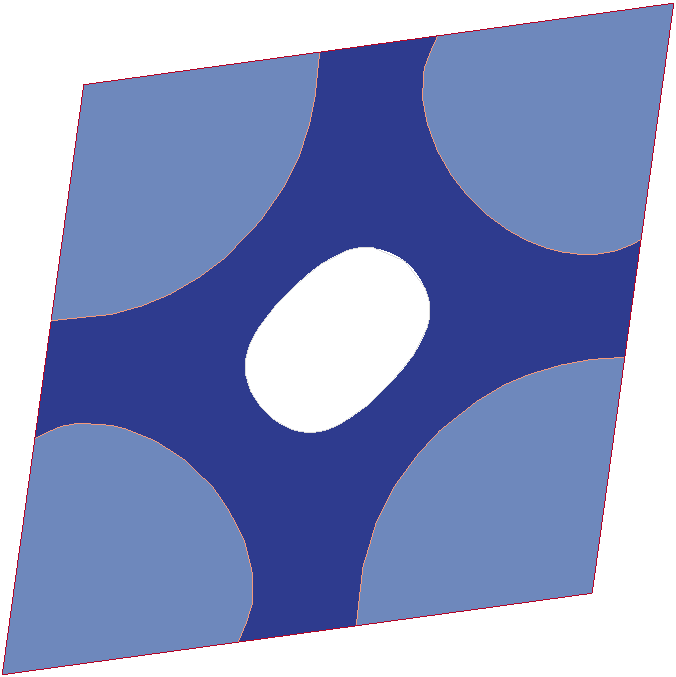
\includegraphics[scale=0.12]{evolve_shear_b.pdf}\label{fig:evolve_shear_b}}
    \\%\hspace{1em}
    \subfloat[$t = 0.65\; t_{\mathrm{end}}$]{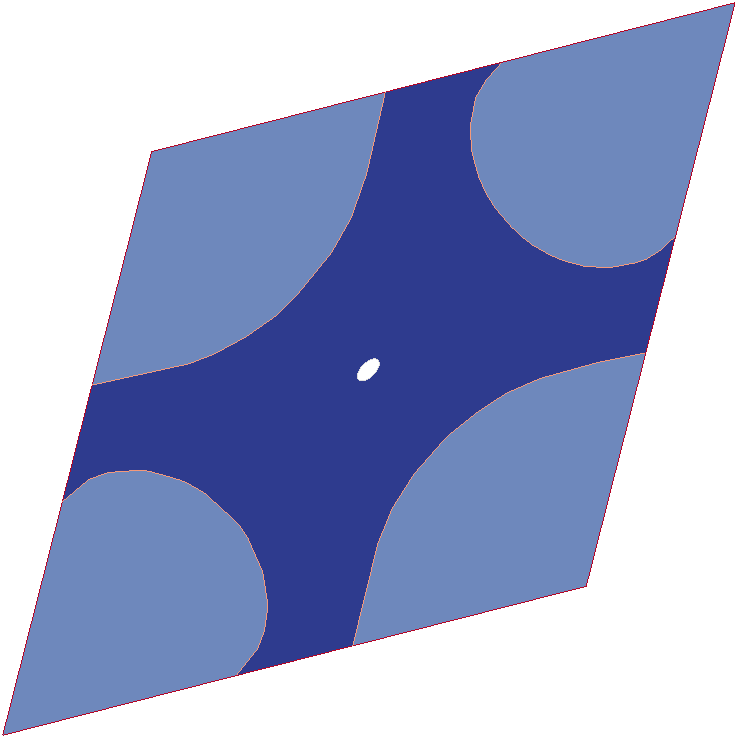
\includegraphics[scale=0.12]{evolve_shear_c.pdf}\label{fig:evolve_shear_c}}
    %\hspace{1em}
    \subfloat[$t = t_{\mathrm{end}}$]{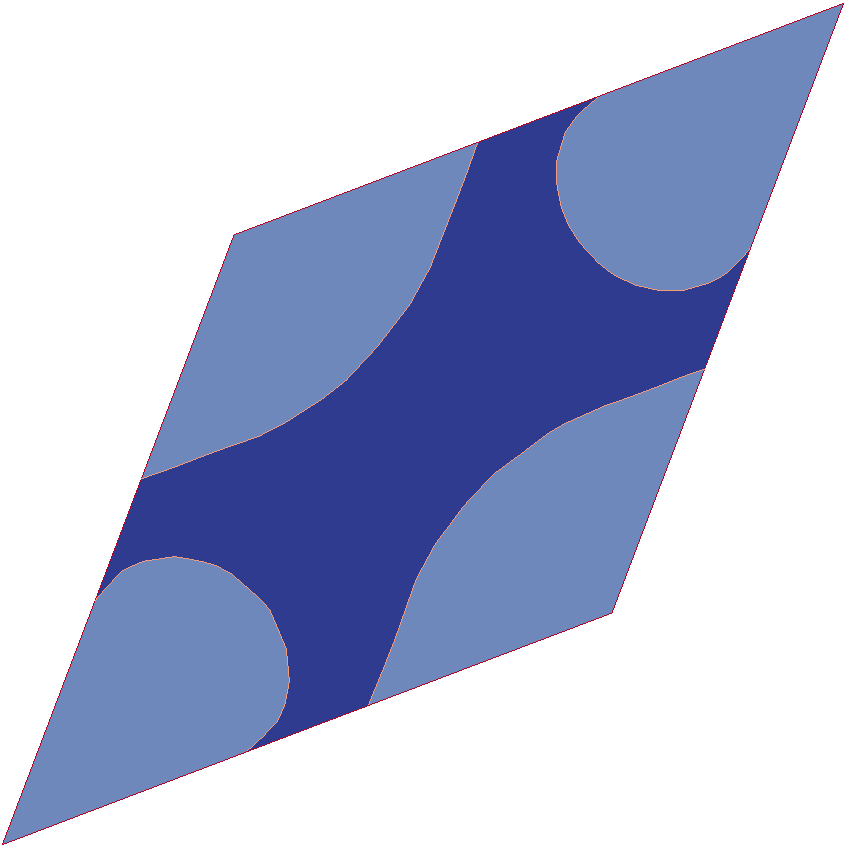
\includegraphics[scale=0.12]{evolve_shear_d.pdf}\label{fig:evolve_shear_d}}
    \caption{Snapshots of evolving RVE subjected to constant macroscopic shear rate, $\bar{\ts d}_\dev \neq \ts 0$, and zero macroscopic pressure, $\bar{p}=0$.}
    \label{fig:evolve_shear}
\end{figure}

Vanishing porosity, i.e. macroscopic incompressibility manifested by $\bar e = 0$ and $\bar{\phi} = 0$, was reached at around $0.69\;t_{\mathrm{end}}$.
After this point in time, the deformation continues but is completely isochoric ($\bar{e} = 0$).
Artifacts from the remeshing of the RVE are noticeable in \figref{fig:evolve_graph} under close examination; however, the overall macroscopic behavior is mostly unaffected.

\begin{figure}[thpb!]
  \centering
%   \tikzsetnextfilename{porosity_over_time}
%   \begin{tikzpicture}
%   \begin{axis}[ yticklabel style={ /pgf/number format/fixed, /pgf/number format/precision=2 },
%                 tick label style={font=\tiny},font=\footnotesize,
%                 height=0.2\textheight, width=1.0\linewidth, xmin=0, xmax=1, ymax=0.175, ymin=-0.015,
%                 legend style={font=\tiny,at={(1,1)},anchor=north east},
%                 xlabel={$t_{\mathrm{end}}$}, ylabel={$\bar{\phi}$}]
%     \addplot[black, densely dashed] table[x=t,y=free] {figures/evolve_gp_porosity.txt};
%     \addlegendentry {$\bar{\ts\sigma}_\dev = \ts 0, \bar{p} = 0$}
%     \addplot[red] table[x=t,y=shear] {figures/evolve_gp_porosity.txt};
%     \addlegendentry {$\bar{\ts d}_\dev \neq \ts 0, \bar{p} = 0$}
%   \end{axis}
%   \end{tikzpicture}
  \includegraphics{porosity_over_time.pdf}
  \caption{Evolution of porosity, $\bar{\phi} = 1-\frac{|\Omega_\Box^\particle|}{|\Omega_\Box|}$,  with time for the RVE subjected to control representing macroscopic shear ($\bar{\ts d}_\dev \neq \ts 0$, $\bar{p} = 0$) and free sintering ($\bar{\ts\sigma}_\dev = \ts 0$, $\bar{p}=0$).}
  \label{fig:evolve_graph}
\end{figure}

We remark that, in the adopted mixed macroscale format, $\bar{\ts d}_\dev$ and $\bar{p}$ are the ``natural'' control variables for the RVE-problems; hence the computation is straight-forward (in contrast to the situation of ``free sintering'' discussed subsequently).

\subsection*{Free sintering ($\bar{\ts\sigma} =\ts 0$)}

In the next series of RVE-computations, the unit cell was subjected to zero macroscopic stress, i.e. $\bar{\ts\sigma} = \ts 0$. Snapshots of the evolving RVE-configuration are given in \figref{fig:evolve_free}, and the corresponding porosity evolution is shown in \figref{fig:evolve_graph}.
Like in the case of macroscopic shear, a fully dense state was reached at around $0.69\;t_{\mathrm{end}}$. However, all deformation stops at this point (which is in contrast to the previously considered case of macroscopic shear).

\begin{figure}[thpb!]
    \centering
    \subfloat[$t = 0$]{
\includegraphics[scale=0.12]{evolve_free_a.pdf}\label{fig:evolve_free_a}}
    \hspace{1em}
    \subfloat[$t = 0.45\; t_{\mathrm{end}}$]{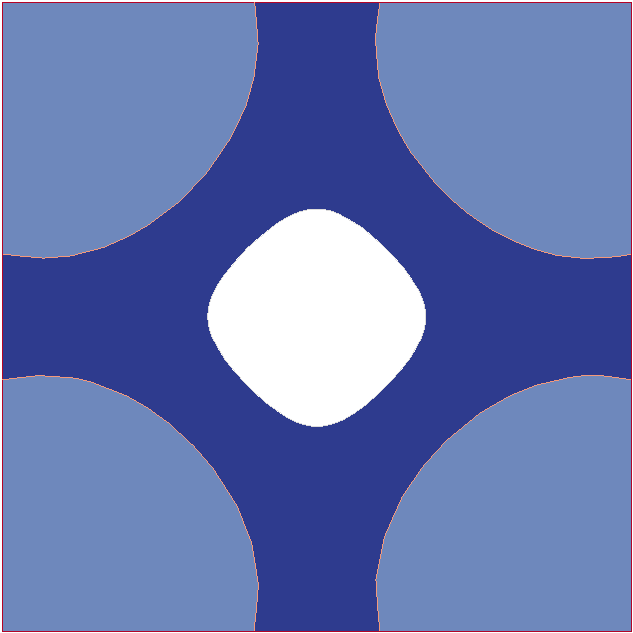
\includegraphics[scale=0.12]{evolve_free_b.pdf}\label{fig:evolve_free_b}}
    \\%\hspace{1em}
    \subfloat[$t = 0.65\; t_{\mathrm{end}}$]{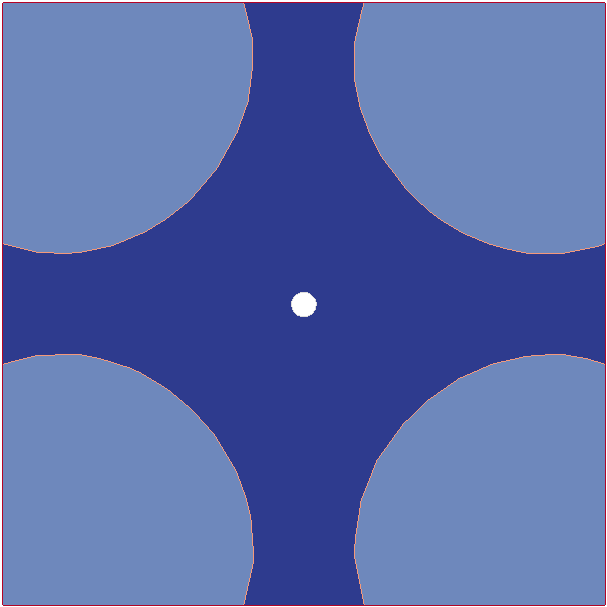
\includegraphics[scale=0.12]{evolve_free_c.pdf}\label{fig:evolve_free_c}}
    \hspace{1em}
    \subfloat[$t = t_{\mathrm{end}}$]{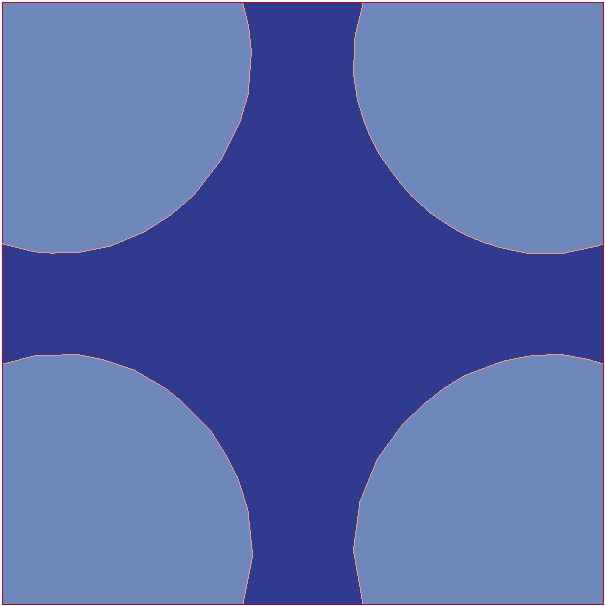
\includegraphics[scale=0.12]{evolve_free_d.pdf}\label{fig:evolve_free_d}}
    \caption{Snapshots of evolving RVE subjected to zero macroscopic stress, $\bar{\ts \sigma}_\dev = \ts 0$ and $\bar{p}=0$.}
    \label{fig:evolve_free}
\end{figure}

% In \figref{fig:evolve_rve} one can see the new boundary condition which prescribes both a constant macroscopic shear and pressure on the RVE,
% and \figref{fig:evolve_graph} shows that a fully dense RVE was reached at around $0.69 t_{\mathrm{end}}$, at which point all volumetric change stopped, while the constant shear rate was still applied.
% The effect of the Dirichlet boundary condition clearly visible in the sheared state.
% The homogenized shear stress is nearly constant throughout the entire simulation.
% Artifacts from remeshing of the RVE is noticeable in \figref{fig:evolve_graph}, however, the overall macroscopic behavior is mostly unaffected.

We remark that prescribing $\bar{\ts\sigma}_\dev$ and $\bar{p}$ represents a situation of ``stress control'' by which macroscale iterations must be carried out on $\bar{\ts d}_\dev$ in order to ensure the prescribed value $\bar{\ts\sigma}_\dev = \ts 0$.
Hence, the macroscale algorithmic tensors are exploited in the corresponding Newton iterations.

\subsection*{FE\textsuperscript{2}-simulation}
\todo{REV} In the last numerical example, we show a fully coupled FE\textsuperscript{2}-simulation, starting from an inhomogeneous initial porosity.
\begin{figure}[thpb!]
\centering
 \includegraphics[width=\linewidth]{figures/evolve_macro_a.pdf} \\
 \includegraphics[width=\linewidth]{figures/evolve_macro_b.pdf} \\
 \includegraphics[width=\linewidth]{figures/evolve_macro_c.pdf}
 \caption{Snapshots of the macroscopic domain with two selected RVE's throughout the densification process.}
 \label{fig:evolve_macro}
\end{figure}
\figref{fig:evolve_macro} shows how the relative density evolves from the initial state, halfway through, to the fully dense product.
The final macroscopic shape distortion is noticeable.
In this simulation, 4 integration points are used for every macroscopic element.
Zoomed-in on the right side of the macroscopic domain, RVEs in two selected integration points are shown.
They undergo successive change of both volume and shape (although the shear deformation is hardly noticeable in the Figure).

\section{Conclusions and outlook}\label{sec:conlusions}

By introducing the mixed variational ($\bar{\ts v},\bar{p}$)-format of the macroscale problem, we can ensure a ``seamless'' transition from the macroscopically compressible to the incompressible response.
Hence, there is no need to change the computational algorithm when the simulation is taken beyond the state of a fully dense macroscopic response (in some spatial point in the macro-domain).
Without such a mixed formulation, the macroscopic ATS-tensor would become unbounded at the transition state.
\todo{REV} In other words, the ``naive'' method described in \figref{fig:box1} would break down halfway through the simulation shown in \figref{fig:evolve_macro}, when any RVE becomes fully dense, while the method in \figref{fig:box2} can continue to a complete dense state without numerical singularities.
% A further advantage of the present formulation is that it allows for more complex constitutive models than the simple isotropic viscous model adopted in this work; one example of added complexity is when $\ts\sigma_\dev$ depends on the intrinsic pressure $p$ in addition to $\ts d_\dev$ (which is the case for anisotropic response due to applied shear rate).
%In any case we define $\bar{p}$ as the negative mean of $\ts\sigma$.

The additional variable in the RVE-problem, as compared to the standard format of Stokes' problem when $\bar{\ts d}$ is the single variable that represents prolongation from the macroscale to the subscale, is $\bar e$. An additional constraint equation is added to ensure that the subscale pressure is homogenized to $p$ in a variationally consistent fashion, whereby the test function is $\delta\bar e\in\set{R}$.
Hence, symmetry is preserved of  the linearized RVE-problem due to the variational format of the ``Galerkin-type''.
The extra computational cost for including $\bar e$ is, indeed, very small in the chosen monolithic format.

As an outlook to future developments, the new mixed RVE-format will be adopted in conjunction with micro-periodic and Neumann boundary conditions.
It would also be of interest to extend the classical strong format of micro-periodicity to a weak variational setting, cf. Larsson et al. \cite{Larsson_etal2011}.
A major advantage is that the subscale FE-mesh does not need to be periodic, which is particularly beneficial in a context of adaptive mesh (re)generation.

The microstructural properties of the ``green body'', i.e. before the sintering process starts, should be represented in a more realistic way than is presently the case.
For example, the RVE should be generated from a given statistical distribution of particle size and shape.
Parameter variations should be carried out of the various geometrical and constitutive properties.
In order to make (inverse) parameter identification meaningful, it is necessary to extend the description of the subscale geometry to three dimensions in the future, although this may represent a major increase in complexity and computational demand.

\todo{REV} All code for the simulations shown in the examples is available in the open source finite element code OOFEM at \texttt{http://www.oofem.org}.


%%%%%%%%%%%%%%%%%%%%%%%%%%%%%%%%%%%%%%%%%%%%%%%%%%%%%%%% REFERENCES %%%%%%%%%%%%%%%%%%%%%%%%%%%%%%%%%%%%%%%%%%%%%555
%\clearpage
\section*{References}
\bibliographystyle{elsarticle-num}
\bibliography{Boundary_representation,Boundary_potentials,Multiscale,FEM_Software,Sintering,Mesh}
%\bibliographystyle{plain}
%\printbibliography



\appendix
%\section{Mathematical Details}
\section{RVE-problem}\label{appendix:RVE}

The weak format of equilibrium for an RVE is
%--------------------------------------------------------------------
\begin{equation}
    \int_{\Omega^\particle_\Box} \ts{\sigma} \dprod \left[\delta \ta{v}\outerp\diff\right] \dif v =
    \int_{\Gamma_\Box\cup\Gamma_\Box^\pore} \ta{t} \cdot \delta\ta{v} \dif a
\label{eq280}
\end{equation}
%-------------------------------------------------------------------------------
for suitable choice of test functions $\delta \ta{v}$. Testing \eqref{eq280} with $\delta \ta{v}^\fluct$, we directly obtain
%--------------------------------------------------------------------
\begin{equation}
    \int_{\Omega^\particle_\Box} \ts{\sigma} \dprod \left[\delta \ta{v}^\fluct\outerp\diff\right] \dif v =
    \int_{\Gamma_\Box^\pore} \ta{t}_\surf \cdot \delta\ta{v}^\fluct \dif a
\label{eq281}
\end{equation}
%-------------------------------------------------------------------------------
which is precisely \eqref{eq:rve_problem_new_v}. Next, testing \eqref{eq280} with $\ta{v}^\macro_\vol(\delta\bar{e})$, we obtain
%--------------------------------------------------------------------
\begin{equation}
    - \left[\int_{\Omega^\particle_\Box} p  \dif v \right]\delta\bar{e} =
    \left[\int_{\Gamma_\Box^\pore} \ta{t}_\surf \cdot \ta{x}_\mean \dif a\right]\delta\bar{e}
    - |\Omega_\Box|\bar{p}\,\delta\bar{e}
\label{eq282}
\end{equation}
%-------------------------------------------------------------------------------
where it was used that $[\ta{x}_\mean\outerp\diff]=\frac{1}{3}\ts{I}$, $p=-\frac{1}{3}\ts{I}\dprod\ts{\sigma}$ and
%--------------------------------------------------------------------
\begin{equation}
    \bar{p} = - \frac{1}{|\Omega_\Box|} \int_{\Gamma_\Box} \ta{t} \cdot \ta{x}_\mean \dif a =
     - \underbrace{\left[\frac{1}{|\Omega_\Box|} \int_{\Gamma_\Box} \ta{t} \outerp [\ta{x}-\bar{\ta{x}}] \dif a\right]}_{\displaystyle\bar{\ts\sigma}}  \dprod \frac{1}{3}\ts{I}
\end{equation}
%-------------------------------------------------------------------------------
Dividing \eqref{eq282} by $|\Omega_\Box|$, we obtain \eqref{eq:rve_problem_new_d}.

\section{Base dyadics in sensitivity problem}

The orthonormal base $\ts E_i$ can be chosen in a cartesian basis, in 2D, as
\begin{align}
 \ts E_1 = \frac{1}{\sqrt{2}}\begin{bmatrix} 1 & 0\\ 0 & -1\end{bmatrix}\quad \ts E_2 = \frac{1}{\sqrt{2}}\begin{bmatrix} 0 & 1\\ 1 & 0\end{bmatrix}
\end{align}
and in 3D, as
\begin{equation}
\begin{gathered}
 \ts E_1 = \frac{1}{\sqrt{6}}\left[\begin{smallmatrix} 2 & 0 & 0\\ 0 & -1 & 0\\ 0 & 0 & -1\end{smallmatrix}\right],\;
 \ts E_2 = \frac{1}{\sqrt{2}}\left[\begin{smallmatrix} 0 & 0 & 0\\ 0 & 1 & 0 \\ 0 & 0 & -1\end{smallmatrix}\right],\\
 \ts E_3 = \frac{1}{\sqrt{2}}\left[\begin{smallmatrix} 0 & 1 & 0\\ 1 & 0 & 0 \\ 0 & 0 & 0\end{smallmatrix}\right],\;
 \ts E_4 = \frac{1}{\sqrt{2}}\left[\begin{smallmatrix} 0 & 0 & 1\\ 0 & 0 & 0 \\ 1 & 0 & 0\end{smallmatrix}\right],\;
 \ts E_5 = \frac{1}{\sqrt{2}}\left[\begin{smallmatrix} 0 & 0 & 0\\ 0 & 0 & 1 \\ 0 & 1 & 0\end{smallmatrix}\right]
\end{gathered}
\end{equation}


\section{Symmetry of the macro-scale problem}

In order to prove symmetry of the macroscale tangent problem it is sufficient to show that it is possible to construct a potential $\bar\Pi\{\bar{\ts d}_\dev,\bar p\}$ with the properties
%-----------------------------------------------------------------------------------------------------------
\begin{align}
 \pd{\bar\Pi}{\bar{\ts d}_\dev} = \bar{\ts\sigma}_\dev, \quad \pd{\bar\Pi}{\bar p} = \bar{e}.
 \label{eq:A1}
\end{align}
%--------------------------------------------------------------------------------------------------
from which it follows directly that
%--------------------------------------------------------------------------------------------------
\begin{align}
 \bar{\tf E}_\ded \defeq \pd{\bar{\ts\sigma}_\dev}{\bar{\ts d}_\dev} = \frac{\partial^2 \bar{\Pi}}{\partial\bar{\ts d}_\dev \outerp \partial\bar{\ts d}_\dev}
\end{align}
%--------------------------------------------------------------------------------------------------
and
%--------------------------------------------------------------------------------------------------
\begin{align}
 \bar{\ts E}_\dep = \pd{\bar{\ts\sigma}_\dev}{\bar{p}} = \frac{\partial^2 \bar{\Pi}}{\partial\bar{\ts d}_\dev \partial\bar{p}} = \pd{\bar{e}}{\bar{\ts d}_\dev} \defeq \bar{\ts C}_\ded.
\end{align}
%--------------------------------------------------------------------------------------------------
We note that that the ``tangent stiffness'' tensor $\bar{\tf E}_\ded$  is symmetrical.

In order to show \eqref{eq:A1}, we start by assuming that it is possible to establish the subscale potential $\Pi_\Box(\bar{\ts d}_\dev,\bar p;\ta v^\fluct,p,\bar{e})$, for given macroscale values $\bar{\ts d}_\dev$, $\bar p$, such that the RVE-problem in \eqref{eq:rve_problem_new} can be stated as
%----------------------------------------------------------------------------------------------------
\begin{subequations}\label{eq:A2}%\label{eq:potential_rve_problem}
\begin{alignat}{5}
\label{eq:A2a}&\Pi'_{\Box,\ta v^\fluct}(\bullet; \delta\ta v^\fluct,p,\bar{e})  &&= 0 \quad && \forall\; \delta\ta v^\fluct &&\in \set{V}_\Box^{(\Dirichlet)}\\
\label{eq:A2b}&\Pi'_{\Box, p^\fluct}(\bullet; \ta v^\fluct,\delta p,\bar{e})    &&= 0 \quad && \forall\; \delta p    &&\in \set{P}_\Box\\
\label{eq:A2c}&\Pi'_{\Box, \bar{e}}(\bullet; \ta v^\fluct,p,\delta\bar{e}) &&= 0 \quad && \forall\; \delta\bar{e} &&\in \set{R}
\end{alignat}
\end{subequations}
%--------------------------------------------------------------------------------------------------------
More explicitly, we define
%-------------------------------------------------------------------------------------------------------------
\begin{align}
 \label{eq:A3}\Pi_\Box(\bar{d}_\dev,\bar p, \ta v^\fluct,p,\bar{e}) = \Psi_\Box(\ta v) + b_\Box(p,\ta v) - l_\Box^\pore(\ta v) + \bar{p}\,\bar{e}
\end{align}
%-------------------------------------------------------------------------------
where we introduced the subscale free energy $\Psi_\Box(\ta v)$ such that
%------------------------------------------------------------------------------------
\begin{align}
 \label{eq:A4}\Psi_\Box'(\ta v;\delta\ta v) = a_\Box(\ta v;\delta\ta v)
\end{align}
%-------------------------------------------------------------------------------------------
and used tacitly the parametrization of the velocity
%---------------------------------------------------------------------------------------------
\begin{align}
 \ta v=\ta v(\bar{\ts d}_\dev,\bar{e},\ta v^\fluct) = \bar{\ts d}_\dev\cdot[\ta x-\bar{\ta x}] + \bar{e} \ta x_\mean + \ta v^\fluct.
\end{align}
%-------------------------------------------------------------------------------------------
It thus follows trivially that \eqref{eq:A2} is precisely the RVE-problem stated in \eqref{eq:rve_problem_new}.

Now, let us define the macroscale potential $\bar\Pi$ as follows
%---------------------------------------------------------------------------------------------------------
\begin{align}
 \label{eq:A5}\bar{\Pi}\{\bar{\ts d}_\dev,\bar p\} \defeq \Pi_\Box(\bar{\ts d}_\dev,\bar{p},\ta v^\fluct\{\bar{\ts d}_\dev,\bar{p}\}, p\{\bar{\ts d}_\dev,\bar{p}\},\bar{e}\{\bar{\ts d}_\dev,\bar{p}\})
\end{align}
%----------------------------------------------------------------------------------------------
where we tacitly account for the implicit relations $\ta v^\fluct\{\bar{\ts d}_\dev,\bar{p}\}$, $p^\fluct\{\bar{\ts d}_\dev,\bar{p}\}$, and $\bar{e}\{\bar{\ts d}_\dev,\bar{p}\}$ via the solution of the RVE-problem \eqref{eq:A2} for given values of (the macroscale variables) $\bar{\ts d}_\dev$ and $\bar{p}$.
Using the chain rule of differentiation and using \eqref{eq:A2}, we then obtain the identities
%-------------------------------------------------------------------------------------------
\begin{align}
 \label{eq:A6}\pd{\bar\Pi}{\bar{\ts d}_\dev} = \pd{\Pi_\Box}{\bar{\ts d}_\dev}\bigg|_{\bar{p},\ta v^\fluct,p, \bar{e}}, \quad
  \pd{\bar\Pi}{\bar{p}} = \pd{\Pi_\Box}{\bar{p}}\bigg|_{\bar{\ts d}_\dev,\ta v^\fluct,p,\bar{e}}
\end{align}
%-------------------------------------------------------------------------------------------------------
However, from the construction of the functional $\Pi_\Box$ in \eqref{eq:A3}, we obtain
%-------------------------------------------------------------------------------------------
\begin{subequations}\label{eq:A7}
\begin{align}
\nonumber \pd{\Pi_\Box}{\bar{\ts d}_\dev} \dprod \dif \bar{\ts d}_\dev &= a_\Box(\ta v; \dif \bar{\ts d}_\dev\cdot[\ta x-\bar{\ta x}]) + \\
  &\underbrace{b_\Box(\dif\bar{\ts d}_\dev\cdot[\ta x-\bar{\ta x}]) }_{=0}
    - l_\Box^\pore(\dif\bar{\ts d}_\dev\cdot[\ta x-\bar{\ta x}]) \label{eq:A7a}\\
\label{eq:A7b}
 \pd{\Pi_\Box}{\bar{p}} \dif \bar{p} &= \bar{e} \dif\bar{p}
\end{align}
\end{subequations}
%--------------------------------------------------------------------------------------------------------
and with \eqref{eq:d_dev_base} we obtain
%--------------------------------------------------------------------------------------------------------
\begin{align}
\label{eq:A8}
 a_\Box(\ta v;\dif\bar{\ts d}_\dev\cdot[\ta x-\bar{\ta x}]) &= \sum_{i=1}^{n_{\mathrm{B}}} a_\Box(\ta v;\ts E_i\cdot[\ta x-\bar{\ta x}])\ts E_i \dprod \dif{\ts d}_\dev\\
\label{eq:A9}
 l_\Box^\pore(\dif\bar{\ts d}_\dev\cdot[\ta x-\bar{\ta x}]) &= \sum_{i=1}^{n_{\mathrm{B}}} l_\Box^\pore(\ts E_i\cdot[\ta x-\bar{\ta x}])\ts E_i \dprod \dif{\ts d}_\dev
\end{align}
%--------------------------------------------------------------------------------------------------------------------------
Next, we can combine \eqref{eq:s_dev_base} with \eqref{eq:sigma_bar_dev_hom} to obtain % \todo{Where?}
%----------------------------------------------------------------------------------------------------------------
\begin{align}
\label{eq:A10}
 \bar{\ts\sigma}_\dev = \sum_{i=1}^{n_{\mathrm{B}}} [a_\Box(\ta v;\ts E_i\cdot[\ta x-\bar{\ta x}]) - l_\Box^\pore(\ts E_i\cdot[\ta x-\bar{\ta x}]) ] \ts E_i
\end{align}
%--------------------------------------------------------------------------------------
and combining this result with \eqref{eq:A8} and \eqref{eq:A9}, we may rephrase \eqref{eq:A6} as
%-------------------------------------------------------------------------------------------
\begin{align}
\label{eq:A11}
 \pd{\Pi_\Box}{\bar{\ts d}_\dev}\bigg|_{\bar{p},\ta v^\fluct,p,\bar{e}} = \bar{\ts\sigma}_\dev \dprod \dif\bar{\ts d}_\dev
\end{align}
%------------------------------------------------------------------------------------------------
Finally, combining \eqref{eq:A11} and \eqref{eq:A7b} with \eqref{eq:A6}, we obtain the desired properties in \eqref{eq:A1}.
Hence, symmetry is proven.

\end{document}
